\documentclass[oneside]{fast-nuces-bs}

\usepackage{mathptmx}% Times Roman font
\usepackage[T1]{fontenc}
\usepackage{sectsty}
\usepackage{tikz-uml}
\usepackage{url}
\usepackage{titlesec}
\usepackage{booktabs,longtable,array,enumitem,float,multirow}
\usepackage{pdflscape}
\usetikzlibrary{arrows.meta,positioning,shapes.geometric,shapes.multipart,fit,calc,backgrounds}
\newcolumntype{P}[1]{>{\raggedright\arraybackslash}p{#1}}

% Information about the report
%%%%%%%%%%%%%%%%%%%%%%%%%%%%%%%%%%%%%%%%%%%%%%%%%%%%%%%%%%%%%%%%%%%%%%%%%%%%%%%
\department{FAST School of Computing}
\faculty{Computer Science}
\degreeyear{2026}
\degreemonth{December}
\degreename{Computer Science}
\campuscity{Islamabad}
\authorone{Moiz Ansari}{23I-0523}
\authortwo{Ruhab Ahmad}{23I-0559}
\authorthree{Saqib Atif}{23I-0769}
\supervisor{Mr. Shehreyar Rashid}
\sessionduration{2023-2027}
\deanname{Dr. Jawwad Shamsi}
\directorname{Dr. Waseem Shahzad}
\hodname{Dr. Arshad Islam}
\fypcoordinatorname{Dr. Behjat}
\title{RetailPulse: Agentic AI for Retail Store Intelligence}
\newcommand{\projecttitle}{RetailPulse: Agentic AI for Retail Store Intelligence}
\newcommand{\studentone}{Moiz Ansari (23I-0523)}
\newcommand{\studenttwo}{Saqib Atif (23I-0769)}
\newcommand{\studentthree}{Ruhab Ahmad (23I-0559)}
%%%%%%%%%%%%%%%%%%%%%%%%%%%%%%%%%%%%%%%%%%%%%%%%%%%%%%%%%%%%%%%%%%%%%%%%%%%%%%%

\hypersetup{hidelinks}
\setlength{\tabcolsep}{4pt}
\setlength{\emergencystretch}{3em}

% Shared diagram styles (all figures are drawn in TikZ so they stay editable and consistent)
\tikzset{
  >={Stealth[length=2.2mm]},
  box/.style={draw, rounded corners=2pt, align=center, font=\small, inner sep=4pt, minimum height=8mm},
  layer/.style={draw, dashed, rounded corners=4pt, inner sep=6pt},
  store/.style={draw, cylinder, shape border rotate=90, aspect=0.18, align=center, font=\small, minimum height=11mm, minimum width=24mm},
  flow/.style={->, thick},
  lbl/.style={font=\scriptsize, fill=white, inner sep=1pt},
}

\begin{document}

\cleardoublepage
\pagenumbering{roman}
\setcounter{page}{1}
\chapter*{Students' Submission}
\addcontentsline{toc}{chapter}{Students' Submission}
\noindent We certify that this report is submitted as the FYP-1 final report for the project titled \textit{\projecttitle}. It describes all work completed up to its submission, including the work presented at the FYP-1 mid evaluation and the work carried out since.
\par\bigskip
\begin{tabular}{P{0.45\textwidth}P{0.45\textwidth}}
Student 1: \studentone & Signature: \rule{0.25\textwidth}{0.4pt}\\[1cm]
Student 2: \studenttwo & Signature: \rule{0.25\textwidth}{0.4pt}\\[1cm]
Student 3: \studentthree & Signature: \rule{0.25\textwidth}{0.4pt}
\end{tabular}

\chapter*{Anti-Plagiarism Statement}
\addcontentsline{toc}{chapter}{Anti-Plagiarism Statement}
The students certify that this report is their own work and that all sources used in preparing it, including external libraries, models, datasets and generative-AI assistance, are acknowledged and referenced.

\chapter*{Authors' Declaration}
\addcontentsline{toc}{chapter}{Authors' Declaration}
We declare that this report documents the work completed by the project team up to the FYP-1 final report. Every measured result in it names the file or command that produced it, synthetic (fixture) results are labelled as such, and contributions, tools, external components and sources are disclosed in Chapter~\ref{ch:mgmt}.

\chapter*{Abstract}
\addcontentsline{toc}{chapter}{Abstract}
Small and mid-sized retailers record CCTV footage but rarely use it to answer operational questions such as whether customers are being attended to and where staff are needed. RetailPulse turns footage from existing cameras into service and staffing information on a CPU-only computer, without biometric identification. A detection and tracking pipeline labels each person as a customer or an employee, and a pose-based check separates a genuine customer--employee interaction from people who are merely close together. Every run is stored as typed events in PostgreSQL. Two business agents read those events through a fixed set of scoped, read-only tools and answer manager questions with claims that are checked against the tools' own figures. A signal policy turns an unattended customer into a staffing event, and a dispatch service sends that task directly to an eligible employee, without a manager approval step. On 14 held-out clips the interaction detector reaches an F1 score of 0.450 (95\,\% interval 0.26--0.63), role classification is correct for all 56 matched tracks, and the pipeline runs at 0.60 times real time on a CPU. The backend has 276 automated tests and the frontend 40, and an end-to-end rehearsal on a synthetic store day passes 8 of 10 acceptance scenarios. Acceptance on real store footage and a deployed backend remain for FYP-2.

\chapter*{Acknowledgments}
\addcontentsline{toc}{chapter}{Acknowledgments}
The project team thanks its supervisor, Mr.\ Shehreyar Rashid, for his guidance and feedback, including the comments from the proposal defence and the mid evaluation that shaped this report. We also thank the faculty of the FAST School of Computing, Islamabad Campus, and our families and peers for their support.

\chapter*{Executive Summary}
\addcontentsline{toc}{chapter}{Executive Summary}
\textbf{Problem.} Store managers cannot easily tell whether customers on the floor are being served, how staff time is split across the floor, or which aisles are left uncovered. CCTV footage holds this information but is watched only after incidents, and commercial retail-analytics products need extra hardware or budgets that small stores do not have.

\textbf{Solution.} RetailPulse reuses existing cameras. A computer-vision pipeline detects and tracks people, labels them as customers or employees from appearance cues, and confirms interactions with a pose check. Results are written to a PostgreSQL event store. On top of the store sit a Customer Behavior agent and an Employee Activity agent, an orchestrator that routes manager questions and checks every number against its source, a signal policy that raises unattended-customer and unstaffed-zone events, and a dispatch service that assigns an eligible employee directly. A Next.js web application gives managers a dashboard and employees a task workspace.

\textbf{Progress since the mid evaluation.} The mid evaluation found the figures and the software requirements specification incorrect. Both were rebuilt for this report: the requirements specification now has sequentially numbered, atomic and testable requirements with measurable non-functional targets (Chapter~\ref{ch:srs}), and every design figure was redrawn from the current code (Chapter~\ref{ch:design}). In the same period the team moved the system from SQLite to PostgreSQL, added the event store, the agents and their grounding checks, direct dispatch with duplicate protection, the four live occupancy categories, map registration, security fixes and continuous integration, and evaluated the vision pipeline on 25 labelled clips.

\textbf{Results.} On held-out clips the interaction detector scores F1 0.450 with role classification correct for all 56 matched tracks; it runs at 0.60 times real time on a CPU. All three continuous-integration jobs pass. A rehearsal of the ten acceptance scenarios on a synthetic store day passes eight; the remaining two need a store map with camera calibration and two human reviewers.

\textbf{Remaining work.} Acceptance on real store footage, a deployed backend, the store floor plan, a second label annotator and the model freeze are planned for FYP-2 (Chapter~\ref{ch:conclusion}).

\tableofcontents
\listoffigures
\listoftables
\chapter*{List of Abbreviations}
\addcontentsline{toc}{chapter}{List of Abbreviations}
\begin{longtable}{P{0.2\textwidth}P{0.7\textwidth}}
\toprule
Abbreviation & Meaning\\
\midrule
API & Application Programming Interface\\
BoT-SORT & Robust Associations Multi-Pedestrian Tracking (the tracker used by the pipeline)\\
CCTV & Closed-Circuit Television\\
CI & Continuous Integration\\
CPU / GPU & Central / Graphics Processing Unit\\
CV & Computer Vision\\
F1 & Harmonic mean of precision and recall\\
FN / FP / TP & False negative / false positive / true positive\\
FR & Functional Requirement\\
HTTP(S) & Hypertext Transfer Protocol (Secure)\\
IoU & Intersection over Union\\
LLM & Large Language Model\\
mAP & mean Average Precision\\
NFR & Non-Functional Requirement\\
PBKDF2 & Password-Based Key Derivation Function 2\\
SRS & Software Requirements Specification\\
UC & Use Case\\
UML & Unified Modeling Language\\
UTC & Coordinated Universal Time\\
YOLO & You Only Look Once (object detector family)\\
\bottomrule
\end{longtable}


\cleardoublepage
\pagenumbering{arabic}
\chapter{Introduction}
\label{ch:intro}

\section{Project Overview}
RetailPulse (\textit{Agentic AI for Retail Store Intelligence}) converts footage from a store's existing CCTV cameras into information a manager can act on: how many customers came in, whether they were attended to, where staff were and where they are needed now. It is designed for small and mid-sized stores, so it runs on an ordinary CPU, needs no new cameras, and never identifies people biometrically.

The system has four parts that build on each other:
\begin{enumerate}
\item a \textbf{vision pipeline} that detects and tracks people, labels each one as a customer or an employee, and confirms customer--employee interactions with a pose check;
\item an \textbf{event store} in PostgreSQL that keeps every run as typed, timestamped records together with camera-health information;
\item an \textbf{agent layer} that answers manager questions from those records and raises operational events, with every figure checked against its source; and
\item a \textbf{web application} with a manager dashboard and an employee task workspace, to which staffing tasks are dispatched directly.
\end{enumerate}

This report is the FYP-1 final report. It covers the whole project to date: the work shown at the mid evaluation on 21 October 2026 and everything completed since.

\section{Problem Statement}
Store managers have no low-cost way to know, during a shift, whether customers on the floor are being attended to and which aisles lack staff. The footage that would answer these questions is already recorded, but nobody watches it in real time, and commercial analytics products require dedicated sensors, subscriptions or analysts that smaller retailers cannot afford.

\section{Motivation}
\begin{itemize}
\item \textbf{Service quality.} A customer who waits without help may leave without buying. A manager who learns about it at the moment it happens can send someone.
\item \textbf{Informed staffing.} Rosters say where staff should be; footage shows where they were. Comparing the two shows coverage gaps.
\item \textbf{Low cost.} Reusing existing cameras and a CPU-only computer removes the capital cost that blocks smaller stores.
\item \textbf{Store-specific service policy.} Service expectations differ between stores: a luxury boutique may not want staff to approach every shopper. All waiting and coverage thresholds are therefore configured per store rather than fixed in code (Section~\ref{sec:srs-constraints}). This answers the generalisability question raised at the proposal defence.
\end{itemize}

\section{Objectives}
Each objective names how it is measured; the measurements are reported in Chapters~\ref{ch:cveval} and~\ref{ch:testing}.
\begin{enumerate}[label=O\arabic*.]
\item Detect people in store footage and classify each tracked person as a customer or an employee without biometric identification. \emph{Measure:} per-track role accuracy on labelled held-out clips.
\item Detect customer--employee interactions and reject close pass-bys. \emph{Measure:} precision, recall and F1 on held-out labelled clips, with and without the pose check, with confidence intervals.
\item Store every analysis run as typed events with provenance and camera health. \emph{Measure:} contract validation of every stored row.
\item Answer manager questions about customers and staff from stored events only. \emph{Measure:} share of answers whose figures match their source tool exactly, and correct refusal of out-of-scope questions.
\item Turn an unattended customer into a task for an eligible employee without manager approval, never twice for the same event. \emph{Measure:} scenario tests for dispatch, no eligible employee, duplicates and blind cameras.
\item Run the vision pipeline on a CPU only. \emph{Measure:} real-time factor on an idle machine.
\item Provide role-based web access for managers and employees. \emph{Measure:} security tests for authentication, role checks and secret handling.
\end{enumerate}

\section{Scope}
\textbf{In scope.}
\begin{itemize}
\item Person detection, tracking and customer/employee classification on recorded or live single-camera video.
\item Interaction detection from body-height-normalised proximity, duration and a pose-based facing check.
\item Entrance footfall, unattended-customer episodes, per-camera heatmaps and pipeline-health records in the event store.
\item Four live occupancy categories for observed map cells: customer, employee, customer and employee, and no one.
\item Customer Behavior and Employee Activity agents, an orchestrator for manager questions, and a narrated digest.
\item Direct dispatch of staffing tasks to eligible employees, with duplicate protection and per-store thresholds.
\item A web application with separate manager and employee workspaces.
\end{itemize}
\textbf{Out of scope.}
\begin{itemize}
\item Facial recognition or any biometric identity.
\item Cross-camera re-identification of the same person (a handoff evaluator exists but no labelled crossings; Section~\ref{sec:cv-limits}).
\item Metric floor distances: a calibrated floor-mapping prototype was built and descoped at the mid evaluation because moving-camera footage gave almost no valid projections.
\item Shelf and product interaction, loss prevention, multi-store operation and automated employee performance rating.
\end{itemize}

\section{Stakeholders and User Classes}
\begin{table}[H]
\centering
\caption{Stakeholders and user classes}\label{tab:stakeholders}
\begin{tabular}{P{0.2\textwidth}P{0.72\textwidth}}
\toprule
Stakeholder & Role and needs\\
\midrule
Store manager & Primary user. Reviews analytics, asks questions, configures the store and resolves alerts. Not assumed to be technical.\\
Employee & Receives and updates staffing tasks and sees only their own shift and tasks.\\
Store owner & Uses summary results for staffing and service decisions.\\
Customers & Appear in footage. Not identified; affected through service quality and privacy.\\
Project team and supervisor & Develop, evaluate and supervise the system.\\
\bottomrule
\end{tabular}
\end{table}

\section{Constraints and Assumptions}
\textbf{Constraints.} No dedicated GPU is available; processing must run on a CPU. The project spans two semesters. The labelled dataset is the team's own recordings from one store with two cameras, because retailers were unwilling to share footage.

\textbf{Assumptions.} Cameras are fixed or move only slightly; staff can be told apart from customers by appearance (for example, uniforms or bibs); each store supplies its roster and its own service thresholds.

\section{Ethical and Legal Considerations}
\textbf{Privacy.} RetailPulse stores no face templates or other biometric identifiers. Track numbers are temporary and per camera, and a tracked employee is never linked to an employee account automatically. Results describe areas and events, not named individuals: the orchestrator refuses questions that ask it to rank or identify people.

\textbf{Fair use.} Staff activity results are decision support, not employee evaluation. An employee standing still while helping a customer is not idle, and an area the camera cannot see is reported as unobserved, never as empty.

\textbf{Law and consent.} Deployment needs a review of local law, store policy and customer notice. Pakistan's personal-data-protection law is listed as draft legislation by the Ministry of IT and Telecommunication~\cite{pakistanMoittLegislation}; the design follows the data-minimisation principle of the GDPR~\cite{gdpr2016}, which does not by itself establish legal compliance.

\section{Report Organisation}
Chapter~\ref{ch:lit} reviews existing products and techniques. Chapter~\ref{ch:srs} is the software requirements specification. Chapter~\ref{ch:design} presents the architecture and design models. Chapter~\ref{ch:impl} describes the implementation in two iterations, Chapter~\ref{ch:cveval} evaluates the vision pipeline, Chapter~\ref{ch:testing} reports testing and acceptance, Chapter~\ref{ch:mgmt} covers project management, and Chapter~\ref{ch:conclusion} concludes and sets out the FYP-2 plan. Appendix~\ref{app:feedback} records how the evaluation feedback was addressed.

\chapter{Literature Review and Existing Solutions}
\label{ch:lit}

\section{Method}
The review covered three areas: commercial retail-analytics products, using their official product descriptions; the published computer-vision methods the pipeline is built from; and recent work on language-model agents that use tools, which shaped how RetailPulse answers questions without inventing figures. Candidate techniques were then tried on the team's own store recordings before being adopted.

\section{Existing Products}
\textbf{RetailNext} describes traffic counting, conversion, staffing and interaction-rate analytics from in-store sensors~\cite{retailnextTraffic}. \textbf{Sensormatic} describes shopper-traffic and journey insights with labour planning~\cite{sensormaticInsights}. \textbf{Amazon Just Walk Out} uses cameras with weight sensors or RFID for checkout-free shopping~\cite{amazonJwo}. These are vendor descriptions; their accuracy, cost and camera compatibility were not independently tested.

\begin{table}[H]
\centering
\caption{Existing products compared with RetailPulse}\label{tab:products}
\begin{tabular}{P{0.18\textwidth}P{0.27\textwidth}P{0.23\textwidth}P{0.24\textwidth}}
\toprule
Product & Documented focus & Hardware & Difference from RetailPulse\\
\midrule
RetailNext & Traffic, conversion, staffing, interaction rate & Vendor sensors & Closed product; RetailPulse reuses existing CCTV on a CPU\\
Sensormatic & Traffic, shopper journeys, labour planning & Vendor sensors & No direct dispatch of staff to a waiting customer described\\
Just Walk Out & Checkout-free shopping & Cameras, shelf weight sensors, RFID & Different goal (checkout); heavy hardware\\
RetailPulse & Service interactions, unattended customers, coverage, direct dispatch & Existing CCTV, CPU only & Inspectable academic prototype; one store evaluated\\
\bottomrule
\end{tabular}
\end{table}

The products already offer substantial analytics, including interaction rates. RetailPulse does not claim these features are absent from the market. Its aim is narrower: an inspectable system that runs on hardware a small store already owns and acts on what it sees by dispatching staff.

\section{Computer-Vision Building Blocks}
\textbf{Detection.} Single-stage YOLO detectors~\cite{redmon2016yolo} have small variants that run on a CPU; the project uses the Ultralytics YOLOv8 implementation~\cite{ultralytics}, exported to OpenVINO~\cite{openvino} for faster CPU inference.

\textbf{Tracking.} SORT~\cite{bewley2016sort} and ByteTrack~\cite{zhang2022bytetrack} link detections into tracks across frames. BoT-SORT~\cite{aharon2022botsort} adds camera-motion compensation and appearance cues, which helps with the slightly moving cameras in the dataset; it is the tracker the pipeline uses. Cross-camera re-identification~\cite{ye2022reid} needs learned appearance embeddings and more compute, and is close to biometric identification, so it is outside the current scope.

\textbf{Pose.} Keypoint models such as YOLO-Pose~\cite{maji2022yolopose} estimate head and shoulder positions in the same single pass as detection. RetailPulse uses head keypoints to check whether two people are facing each other, which separates a conversation from two people walking side by side.

\textbf{Evaluation statistics.} With a small labelled set, a single F1 value is unreliable. The project reports bootstrap confidence intervals~\cite{efron1979bootstrap} resampled over clips, and Cohen's kappa~\cite{cohen1960kappa} for agreement between human reviewers.

\section{Language-Model Agents and Grounding}
Language models can plan and call external tools: ReAct interleaves reasoning with tool calls~\cite{yao2023react}, and Toolformer shows models learning when to call an API~\cite{schick2023toolformer}. The main risk for a store manager is hallucination, where fluent text states figures the data does not support~\cite{ji2023hallucination}. RetailPulse therefore separates the two roles: agents may only call a fixed set of read-only tools, every number in an answer must be a claim that points at a specific metric in a tool result, and an answer whose claims do not match is repaired or refused. The orchestration graph is built with LangGraph~\cite{langgraph}, and the event store uses PostgreSQL~\cite{postgresql}.

\section{Gap Addressed}
Three gaps follow from the review.
\begin{enumerate}
\item \textbf{Interaction versus proximity.} Proximity alone counts two people walking past each other as an interaction. On the held-out clips, adding the pose check in the same run raises precision from 0.346 to 0.391 at the same recall (Chapter~\ref{ch:cveval}).
\item \textbf{Acting, not only reporting.} The reviewed products describe dashboards and staffing plans. RetailPulse turns a waiting customer into a task for a specific eligible employee, with rules that protect zone minimum staffing and prevent duplicate tasks.
\item \textbf{Trustworthy answers.} Manager answers carry their evidence, and missing camera coverage is reported as unknown, never as an empty area.
\end{enumerate}

\section{Complex Computing Problem}
Deriving service analytics from uncontrolled CCTV on a CPU is a complex computing problem in the sense of the programme outcomes:
\begin{itemize}
\item \textbf{Conflicting requirements:} accuracy against CPU throughput, and useful staff analytics against privacy and fair use.
\item \textbf{No single correct definition:} whether two people ``interacted'' has to be defined operationally from distance, orientation and duration, and labellers can disagree about pauses.
\item \textbf{Uncertain inputs:} identity switches, occlusion and blocked cameras mean some observations are unknown, and the system must carry that uncertainty to the manager instead of hiding it.
\item \textbf{Several interacting subsystems:} vision, storage, agents, dispatch and the web tier must agree on identifiers, time and provenance.
\end{itemize}

\chapter{Software Requirements Specification}
\label{ch:srs}

This chapter specifies what RetailPulse must do, following the structure of ISO/IEC/IEEE 29148~\cite{iso29148}. It replaces the requirements chapter of the mid report, which the mid evaluation found incorrect. The main changes are listed in Appendix~\ref{app:req-changes}: requirements are now numbered without gaps, each states a single testable behaviour, non-functional requirements have measurable targets, and implementation progress is reported separately in Chapters~\ref{ch:impl} to~\ref{ch:testing} instead of inside the specification.

\section{Purpose and Product Scope}
RetailPulse analyses footage from a store's existing cameras to detect customers and employees, find customer--employee interactions and unattended customers, show this information to the manager, and assign staff to where they are needed. The specification covers the vision pipeline, the event store, the analytics agents, staff dispatch and the web application.

\section{Product Perspective}
RetailPulse is a self-contained system that uses the store's cameras as input. Figure~\ref{fig:context} shows its context: two human actors, the camera system, and two optional external services. The event store is part of the system, not an external actor.

\begin{figure}[htbp]
\centering
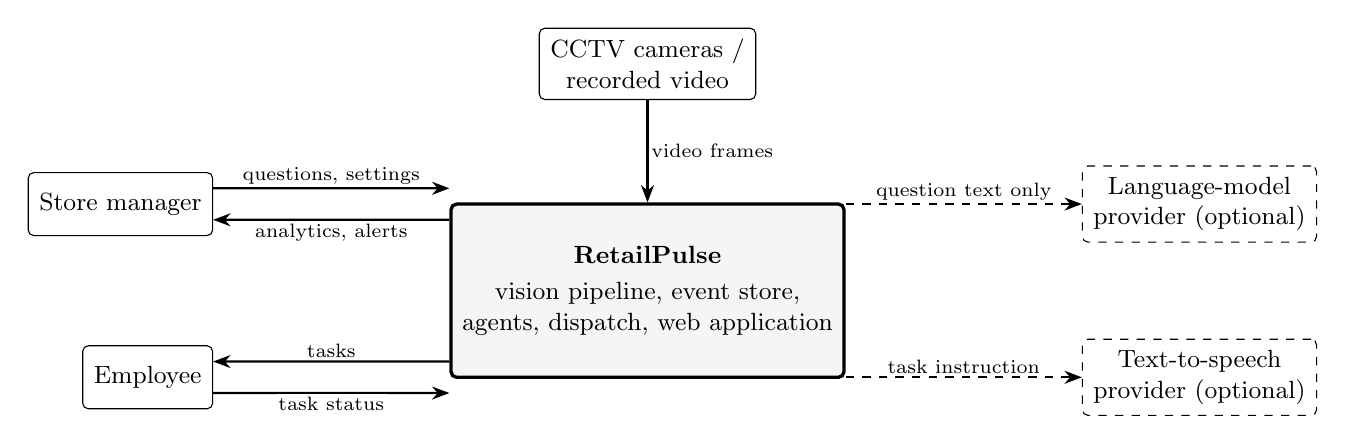
\begin{tikzpicture}[node distance=1.2cm]
\node[box, minimum width=4.6cm, minimum height=2.2cm, very thick, fill=gray!8] (sys) {\textbf{RetailPulse}\\[2pt]vision pipeline, event store,\\agents, dispatch, web application};
\node[box, left=3.0cm of sys, yshift=1.1cm] (mgr) {Store manager};
\node[box, left=3.0cm of sys, yshift=-1.1cm] (emp) {Employee};
\node[box, above=1.3cm of sys] (cam) {CCTV cameras /\\recorded video};
\node[box, right=3.0cm of sys, yshift=1.1cm, dashed] (llm) {Language-model\\provider (optional)};
\node[box, right=3.0cm of sys, yshift=-1.1cm, dashed] (tts) {Text-to-speech\\provider (optional)};
\draw[flow] (cam) -- node[lbl, right] {video frames} (sys);
\draw[flow] ([yshift=2mm]mgr.east) -- node[lbl, above] {questions, settings} ([yshift=1.3cm]sys.west);
\draw[flow] ([yshift=0.9cm]sys.west) -- node[lbl, below] {analytics, alerts} ([yshift=-2mm]mgr.east);
\draw[flow] ([yshift=-0.9cm]sys.west) -- node[lbl, above] {tasks} ([yshift=2mm]emp.east);
\draw[flow] ([yshift=-2mm]emp.east) -- node[lbl, below] {task status} ([yshift=-1.3cm]sys.west);
\draw[flow, dashed] ([yshift=1.1cm]sys.east) -- node[lbl, above] {question text only} (llm.west);
\draw[flow, dashed] ([yshift=-1.1cm]sys.east) -- node[lbl, above] {task instruction} (tts.west);
\end{tikzpicture}
\caption{System context: actors and external services}
\label{fig:context}
\end{figure}

The language-model provider may be used only to choose which agent handles a manager's question; it never supplies figures or chooses tools. The text-to-speech provider turns a task instruction into audio for the employee. Both are optional: without them the system routes questions with fixed rules and shows tasks as text.

\section{User Classes and Characteristics}
\begin{table}[H]
\centering
\caption{User classes}\label{tab:user-classes}
\begin{tabular}{P{0.16\textwidth}P{0.42\textwidth}P{0.32\textwidth}}
\toprule
User class & Characteristics & Access\\
\midrule
Manager & Runs the store; not necessarily technical; uses the dashboard on a laptop or phone. & All analytics, questions, alerts, configuration and system status for their store.\\
Employee & Works on the floor; uses a phone or shared screen. & Own shift, own tasks and own profile only.\\
\bottomrule
\end{tabular}
\end{table}

\section{Operating Environment}
\begin{itemize}
\item Server: a Windows or Linux computer with a multi-core CPU and no GPU, running Python 3.11 and PostgreSQL 17 (local or hosted).
\item Web tier: Next.js 15 on Node.js 20 or later, deployable on Vercel.
\item Clients: current desktop and mobile browsers (Chrome, Edge, Firefox, Safari).
\item Cameras: fixed CCTV cameras providing a video stream or recorded files readable by OpenCV.
\end{itemize}

\section{Design and Implementation Constraints}
\label{sec:srs-constraints}
\begin{enumerate}[label=C\arabic*.]
\item Vision processing must run on a CPU without a GPU.
\item No biometric identifier (face template or identity embedding linked to a person) may be stored.
\item Waiting, staffing, coverage and occupancy thresholds are store configuration, not code constants, so each store can set its own service policy.
\item Agents may read store data only through the fixed read-only analytics tools; they may not run arbitrary database queries.
\item Assigning an aisle task to an employee must not require manager approval.
\item Secrets (session, internal service and provider keys) are read from the environment and never sent to the browser.
\end{enumerate}

\textbf{Assumptions and dependencies.} Staff can be told apart from customers by appearance, such as a uniform or bib. Each store supplies its zones, minimum staffing per zone and a staff roster. A store map with camera calibration points must be supplied before map-cell occupancy can be shown.

\section{Use Case Model}
\label{sec:uc-model}
Figure~\ref{fig:uc-diagram} shows the twelve use cases. The manager is the primary actor for most of them. The employee is primary for viewing and updating their tasks, and secondary for dispatch, where they receive the task. The camera system is the primary actor of the dispatch use case because a closed observation window, not a person, triggers it. Signing in is shared by both human actors. \emph{Generate store digest} always runs analytics questions, so it includes UC-04; updating a task's status is an optional extension of viewing one's tasks.

\begin{figure}[p]
\centering
\begin{tikzpicture}[scale=0.84, transform shape,
  uc/.style={ellipse, draw, align=center, font=\footnotesize, inner xsep=2pt, inner ysep=0pt, minimum width=4.7cm, minimum height=1.0cm},
  assoc/.style={thin},
  dep/.style={->, dashed, thin}]
% system boundary
\draw[rounded corners=3pt, thick] (2.9,0.95) rectangle (15.0,-13.2);
\node[font=\bfseries] at (8.95,0.6) {RetailPulse};
% manager use cases (left column)
\node[uc] (u01) at (5.9,-0.20) {UC-01\\Sign in};
\node[uc] (u03) at (5.9,-1.55) {UC-03\\View dashboard analytics};
\node[uc] (u04) at (5.9,-2.90) {UC-04\\Ask an analytics question};
\node[uc] (u08) at (5.9,-4.25) {UC-08\\Generate store digest};
\node[uc] (u09) at (5.9,-5.60) {UC-09\\View live occupancy};
\node[uc] (u05) at (5.9,-6.95) {UC-05\\Review and resolve alerts};
\node[uc] (u06) at (5.9,-8.30) {UC-06\\Configure store};
\node[uc] (u07) at (5.9,-9.65) {UC-07\\View system status};
\node[uc] (u02) at (5.9,-11.00) {UC-02\\Process store video};
\node[uc] (u12) at (5.9,-12.35) {UC-12\\Dispatch staffing task};
% employee use cases (right column)
\node[uc] (u10) at (12.0,-5.30) {UC-10\\View own tasks and shift};
\node[uc] (u11) at (12.0,-7.15) {UC-11\\Update task status};
% actors
\foreach \name/\x/\y/\txt in {mgr/0.5/-6.1/Manager, cam/0.5/-12.4/{Camera system\\\scriptsize\guillemotleft system\guillemotright}, emp/17.0/-6.8/Employee} {
  \begin{scope}[shift={(\x,\y)}]
    \draw (0,0.95) circle (0.17);
    \draw (0,0.78) -- (0,0.25) (-0.3,0.6) -- (0.3,0.6) (0,0.25) -- (-0.25,-0.15) (0,0.25) -- (0.25,-0.15);
    \node[align=center, font=\footnotesize, below] at (0,-0.15) {\txt};
    \coordinate (\name) at (0,0.5);
  \end{scope}
}
% manager associations
\foreach \u in {u01,u03,u04,u08,u09,u05,u06,u07,u02} { \draw[assoc] (mgr) -- (\u.west); }
% camera associations
\draw[assoc] (cam) -- (u02.west);
\draw[assoc] (cam) -- (u12.west);
% employee associations
\draw[assoc] (emp) -- (u01.east);
\draw[assoc] (emp) -- (u10.east);
\draw[assoc] (emp) -- (u11.east);
\draw[assoc] (emp) -- (u12.east);
% include / extend
\draw[dep] (u08.east) to[out=0, in=0, looseness=1.7] node[right, font=\scriptsize] {\guillemotleft include\guillemotright} (u04.east);
\draw[dep] (u11) -- node[right, font=\scriptsize] {\guillemotleft extend\guillemotright} (u10);
\end{tikzpicture}
\caption{Use case diagram}
\label{fig:uc-diagram}
\end{figure}

\section{Use Case Descriptions}
Each description lists the functional requirements it realises. Steps are numbered so that alternative flows can refer to them.

\newcommand{\ucrow}[2]{#1 & #2\\}
\newenvironment{ucspec}[2]{%
  \begin{longtable}{P{0.2\textwidth}P{0.72\textwidth}}
  \caption{#1}\label{#2}\\
  \toprule
  \endfirsthead
  \toprule
  \endhead
  \bottomrule
  \endfoot}{\end{longtable}}

\begin{ucspec}{UC-01 Sign in}{tab:uc01}
\ucrow{Actors}{Manager or Employee (primary)}
\ucrow{Realises}{FR-01, FR-02, FR-03}
\ucrow{Precondition}{The user has an active account.}
\ucrow{Main flow}{1. The user enters email and password and selects Manager or Employee. 2. The system verifies the password and that the selected role matches the stored role. 3. The system issues a signed session. 4. The system opens the manager dashboard or the employee home page.}
\ucrow{Alternatives}{2a. Wrong password: the system shows an error and counts the failure. 2b. Five failures for the account within 15 minutes: the system locks the account for 15 minutes. 2c. The selected role does not match the stored role: the system refuses the sign-in.}
\ucrow{Postcondition}{The user can reach only the workspace of their role until they sign out or the session expires.}
\end{ucspec}

\begin{ucspec}{UC-02 Process store video}{tab:uc02}
\ucrow{Actors}{Manager (primary); camera system (secondary)}
\ucrow{Realises}{FR-05 to FR-10}
\ucrow{Precondition}{The manager is signed in; the camera or recording is registered.}
\ucrow{Main flow}{1. The manager selects a recording or a live camera and starts analysis. 2. The system admits the job. 3. The system detects, tracks and classifies people and checks candidate interactions with the pose check. 4. The system shows an annotated preview while it runs. 5. The system writes the outputs and stores the run's events with the camera identifier.}
\ucrow{Alternatives}{2a. Two jobs are already running: the system refuses the new job and asks the manager to retry later. 3a. The video cannot be read: the system stops and reports the error without storing partial results as complete.}
\ucrow{Postcondition}{The run's events and camera-health records are in the event store.}
\end{ucspec}

\begin{ucspec}{UC-03 View dashboard analytics}{tab:uc03}
\ucrow{Actors}{Manager (primary)}
\ucrow{Realises}{FR-17}
\ucrow{Precondition}{The manager is signed in and is a member of the store.}
\ucrow{Main flow}{1. The manager opens the dashboard and selects an interval and, optionally, a zone. 2. The system reads footfall, interactions, unattended episodes, coverage and dwell through the analytics tools. 3. The system shows each figure with its unit, evidence and limitations.}
\ucrow{Alternatives}{2a. A source has no data for the interval: the figure is shown as unavailable with the reason, never as zero. 2b. The backend cannot be reached: the dashboard shows an error and does not fall back to sample data.}
\ucrow{Postcondition}{No data is changed.}
\end{ucspec}

\begin{ucspec}{UC-04 Ask an analytics question}{tab:uc04}
\ucrow{Actors}{Manager (primary)}
\ucrow{Realises}{FR-18, FR-19, FR-20}
\ucrow{Precondition}{The manager is signed in and has asked fewer than ten questions in the current minute.}
\ucrow{Main flow}{1. The manager types a question about customers or staff. 2. The system routes it to the Customer Behavior or Employee Activity agent. 3. The agent calls the analytics tools for the dashboard's interval and filters. 4. The system checks every figure against the tool result it cites. 5. The system shows the answer with its figures, citations and limitations.}
\ucrow{Alternatives}{2a. The question asks to rank or identify people, or to take an action: the system refuses. 4a. A figure does not match its source: the agent is asked to repair it once; if it still fails, the claim is dropped. 4b. No supporting evidence: the system says so instead of answering.}
\ucrow{Postcondition}{No store data is changed.}
\end{ucspec}

\begin{ucspec}{UC-05 Review and resolve alerts}{tab:uc05}
\ucrow{Actors}{Manager (primary)}
\ucrow{Realises}{FR-30}
\ucrow{Precondition}{The manager is signed in.}
\ucrow{Main flow}{1. The manager opens Alerts and filters by status, category or severity. 2. The system lists the alerts with their evidence and any related task. 3. The manager resolves an alert. 4. The system records who resolved it and when.}
\ucrow{Alternatives}{3a. The manager assigns a task from the alert: the system applies the dispatch rules of UC-12 to the alert's zone.}
\ucrow{Postcondition}{Resolved alerts move to the resolved list; resolving an alert never cancels a task.}
\end{ucspec}

\begin{ucspec}{UC-06 Configure store}{tab:uc06}
\ucrow{Actors}{Manager (primary)}
\ucrow{Realises}{FR-31, FR-32}
\ucrow{Precondition}{The manager is signed in.}
\ucrow{Main flow}{1. The manager edits zones and their minimum staff, cameras, staff rosters or service thresholds. 2. The system validates the change. 3. The system saves it and applies it to later decisions.}
\ucrow{Alternatives}{2a. Invalid value: the system rejects the change and keeps the previous configuration. 1a. The manager pauses automatic dispatch: later staffing events raise alerts only.}
\ucrow{Postcondition}{The new configuration is used for every decision made after saving.}
\end{ucspec}

\begin{ucspec}{UC-07 View system status}{tab:uc07}
\ucrow{Actors}{Manager (primary)}
\ucrow{Realises}{FR-33}
\ucrow{Main flow}{1. The manager opens System Status. 2. The system shows database and component health, recent dispatch outcomes, and task acknowledgement counts with mean and median times.}
\ucrow{Alternatives}{2a. A component reports no telemetry: it is shown as unknown, not healthy.}
\end{ucspec}

\begin{ucspec}{UC-08 Generate store digest}{tab:uc08}
\ucrow{Actors}{Manager (primary)}
\ucrow{Realises}{FR-21}
\ucrow{Main flow}{1. The manager selects an interval and requests a digest. 2. The system runs the customer and staffing questions of UC-04 for that interval. 3. The system writes the digest sections (traffic, assistance, waiting customers, staff coverage, events raised) from the verified figures. 4. The system lists caveats, including any interval in which a camera was blind.}
\ucrow{Alternatives}{3a. The data is synthetic: the digest says so on its first line.}
\ucrow{Postcondition}{Every number in the digest equals a verified figure.}
\end{ucspec}

\begin{ucspec}{UC-09 View live occupancy}{tab:uc09}
\ucrow{Actors}{Manager (primary)}
\ucrow{Realises}{FR-15, FR-16}
\ucrow{Precondition}{A store map is registered for at least one camera.}
\ucrow{Main flow}{1. The manager opens the spatial view. 2. The system shows each mapped cell in one of the four categories, with the map version and window. 3. The system shows customer, employee and confirmed-interaction layers separately.}
\ucrow{Alternatives}{2a. A cell lacks coverage or has unknown roles: it is masked with the reason, never shown as \emph{no one}.}
\end{ucspec}

\begin{ucspec}{UC-10 View own tasks and shift}{tab:uc10}
\ucrow{Actors}{Employee (primary)}
\ucrow{Realises}{FR-28}
\ucrow{Precondition}{The employee is signed in.}
\ucrow{Main flow}{1. The employee opens their home page. 2. The system shows open tasks first, then shift and zone. 3. When a new task is assigned, the system adds it without a page reload.}
\ucrow{Alternatives}{2a. No open task: the page says so.}
\ucrow{Postcondition}{The employee sees only their own tasks.}
\end{ucspec}

\begin{ucspec}{UC-11 Update task status}{tab:uc11}
\ucrow{Actors}{Employee (primary)}
\ucrow{Realises}{FR-29}
\ucrow{Extends}{UC-10, at the point where the employee selects a task.}
\ucrow{Main flow}{1. The employee acknowledges, starts or completes a task. 2. The system records the new state and its time. 3. The manager sees the change in Alerts and System Status.}
\ucrow{Alternatives}{1a. The employee taps the button twice: the page ignores the second tap until the first update completes. 2a. The task belongs to another employee: the system refuses the update.}
\end{ucspec}

\begin{ucspec}{UC-12 Dispatch staffing task}{tab:uc12}
\ucrow{Actors}{Camera system (primary); Employee (secondary)}
\ucrow{Realises}{FR-11, FR-22 to FR-27, FR-34}
\ucrow{Trigger}{An observation window for a zone closes.}
\ucrow{Main flow}{1. The system reads the zone's unattended episodes, dwell and camera coverage for the window. 2. A customer waited at least the store's threshold without help, so the system raises an unattended-customer event. 3. The system selects an eligible employee. 4. The system creates the task with an instruction and a one-line reason, records the decision and an alert, and delivers the task to the employee. 5. The employee sees the task (UC-10).}
\ucrow{Alternatives}{2a. The camera was blind for more than the allowed share of the window: the event is suppressed and the reason recorded. 3a. No eligible employee: no task is created and the manager is alerted. 3b. The event was already handled: the system reports a duplicate and creates no task. 3c. A task for the zone is still open: the existing task stands. 3d. Dispatch is paused: an alert is raised without a task.}
\ucrow{Postcondition}{At most one task exists per event, and every decision is recorded with its reason.}
\end{ucspec}

\section{Functional Requirements}
Priorities: \textbf{H} (needed for the core service), \textbf{M} (needed for a complete product), \textbf{L} (useful addition).

\begin{longtable}{P{0.085\textwidth}P{0.63\textwidth}P{0.045\textwidth}P{0.13\textwidth}}
\caption{Functional requirements}\label{tab:fr}\\
\toprule
ID & Requirement & Pr. & UC\\
\midrule
\endfirsthead
\toprule
ID & Requirement & Pr. & UC\\
\midrule
\endhead
\bottomrule
\endfoot
\multicolumn{4}{l}{\textit{Accounts and access}}\\
FR-01 & The system shall authenticate users by email and password and issue a signed session that browser scripts cannot read. & H & UC-01\\
FR-02 & The system shall give each user access only to the workspace and data of their stored role, and refuse a sign-in whose selected role differs from the stored role. & H & UC-01\\
FR-03 & The system shall lock an account for 15 minutes after five failed sign-in attempts within 15 minutes. & H & UC-01\\
FR-04 & The system shall let a manager invite an employee through a single-use link that expires after seven days. & M & UC-06\\
\multicolumn{4}{l}{\textit{Video analysis}}\\
FR-05 & The system shall detect people in sampled frames of a recorded video or a live camera stream. & H & UC-02\\
FR-06 & The system shall give each detected person a track identifier that stays the same while the person remains visible to the same camera. & H & UC-02\\
FR-07 & The system shall classify each track as customer or employee and record the classification score. & H & UC-02\\
FR-08 & The system shall nominate an interaction when an employee and a customer stay within the configured body-height-normalised distance for at least the configured duration. & H & UC-02\\
FR-09 & The system shall confirm a nominated interaction only when the pose check finds the two people facing each other, and otherwise mark it rejected or unverified. & H & UC-02\\
FR-10 & The system shall write, for each run, an annotated video and structured files of detections, people and interactions. & M & UC-02\\
\multicolumn{4}{l}{\textit{Event store}}\\
FR-11 & The system shall store each run's tracks, role decisions, interactions, zone dwell, footfall, queue samples, unattended episodes, camera health and heatmaps, each with run, store, camera and zone identifiers and UTC start and end times. & H & UC-02, UC-12\\
FR-12 & The system shall record an unattended episode when a customer waits at least the store's unattended threshold without a confirmed interaction. & H & UC-12\\
FR-13 & The system shall count entries and exits across a configured entrance line, counting each track's crossing once. & M & UC-03\\
FR-14 & The system shall record each camera's health every minute: frame rate, mean confidence, unknown-role share, identity churn and frozen or dark frames. & H & UC-07\\
\multicolumn{4}{l}{\textit{Live occupancy}}\\
FR-15 & The system shall place each observed map cell in each window in exactly one of four categories (customer, employee, customer and employee, no one), or mask it with a quality reason when coverage or role evidence is insufficient. & M & UC-09\\
FR-16 & The system shall change a cell's displayed category only after the new category holds for the configured number of consecutive windows. & M & UC-09\\
\multicolumn{4}{l}{\textit{Analytics and questions}}\\
FR-17 & The system shall show the manager, for a selected interval and zone, footfall, interactions, unattended episodes, staff coverage and dwell, each with its evidence and limitations. & H & UC-03\\
FR-18 & The system shall answer a manager's question about customers or staff using only the five read-only analytics tools. & M & UC-04\\
FR-19 & The system shall check every figure in an answer against the tool metric it cites and remove any figure that does not match. & H & UC-04\\
FR-20 & The system shall refuse questions that ask it to rank or identify individuals or to perform an operational action. & H & UC-04\\
FR-21 & The system shall produce a store digest for a selected interval in which every number is a verified figure and synthetic data is labelled. & M & UC-08\\
\multicolumn{4}{l}{\textit{Operational events and dispatch}}\\
FR-22 & The system shall raise an unattended-customer event for a zone when at least one unhelped wait in the window reaches the store's minimum wait. & H & UC-12\\
FR-23 & The system shall raise an unstaffed-zone event when a zone's staffed share of open time falls below the store's minimum while customers are present. & M & UC-12\\
FR-24 & The system shall suppress both events, recording the reason, when the camera's unknown-observation share in the window exceeds the store's maximum. & H & UC-12\\
FR-25 & The system shall select only an employee who is active, rostered, available, without an open task and not in an interaction, and whose departure keeps their own zone at or above its minimum staff. & H & UC-12\\
FR-26 & The system shall rank eligible employees by: staff of the target zone, then floaters, then the zone with the most spare staff. & M & UC-12\\
FR-27 & The system shall deliver the task to the selected employee with an instruction and a one-line reason, without manager approval. & H & UC-12\\
FR-28 & The system shall show each employee their open tasks, shift and zone, and add newly assigned tasks without a page reload. & H & UC-10\\
FR-29 & The system shall record each task status change (acknowledged, in progress, completed or declined) with its time. & H & UC-11\\
\multicolumn{4}{l}{\textit{Alerts, configuration and status}}\\
FR-30 & The system shall let a manager filter alerts and resolve them, recording who resolved each alert and when. & M & UC-05\\
FR-31 & The system shall let a manager configure zones with minimum staff, cameras, rosters and service thresholds, rejecting invalid values. & H & UC-06\\
FR-32 & The system shall let a manager pause automatic dispatch, after which staffing events raise alerts only. & M & UC-06\\
FR-33 & The system shall show component health, recent dispatch outcomes and task acknowledgement times. & L & UC-07\\
FR-34 & The system shall create at most one task per staffing event, returning the earlier decision when the same event is received again. & H & UC-12\\
\end{longtable}

\section{Non-Functional Requirements}
Each requirement has a measurable target and a verification method. Measured results are reported in Chapters~\ref{ch:cveval} and~\ref{ch:testing}. The reference machine is a laptop with a multi-core CPU, no GPU and nothing else running.

\begin{longtable}{P{0.095\textwidth}P{0.17\textwidth}P{0.4\textwidth}P{0.24\textwidth}}
\caption{Non-functional requirements}\label{tab:nfr}\\
\toprule
ID & Quality & Requirement and target & Verification\\
\midrule
\endfirsthead
\toprule
ID & Quality & Requirement and target & Verification\\
\midrule
\endhead
\bottomrule
\endfoot
NFR-01 & Performance & The vision pipeline shall process recorded video at no less than 0.5 times real time on the reference machine with default sampling. & Timed benchmark on the held-out clips on an idle machine.\\
NFR-02 & Accuracy & Interaction detection shall reach F1 of at least 0.40 on held-out labelled clips, reported with a 95\,\% confidence interval. & Benchmark on the held-out set; clip bootstrap.\\
NFR-03 & Accuracy & Customer/employee classification shall be correct for at least 95\,\% of matched tracks on held-out clips. & Role benchmark against reviewed person labels.\\
NFR-04 & Reliability & Replaying any staffing event shall create zero additional tasks. & Duplicate-event scenario and unit tests.\\
NFR-05 & Integrity & Every stored event row shall carry non-empty run, store, camera and zone identifiers and end no earlier than it starts. & Contract check \texttt{validate()} on every run.\\
NFR-06 & Honesty of data & Missing camera coverage shall never be reported as zero activity or as an empty area. & Blind-camera scenario; occupancy masking tests.\\
NFR-07 & Security & Passwords shall be stored with PBKDF2-SHA256 using at least 600\,000 iterations~\cite{owaspPasswords} and shall be at least eight characters. & Unit tests on hashing and sign-up validation.\\
NFR-08 & Security & The backend shall reject every request without the internal service secret and shall refuse to start with a missing or default secret outside development mode. & Security tests; startup test.\\
NFR-09 & Security & Each manager shall be limited to ten questions per minute. & Rate-limit test.\\
NFR-10 & Privacy & No face template, identity embedding linked to a person, or employee account identity derived from a CV track shall be stored. & Schema and code review.\\
NFR-11 & Usability & Every manager page shall be reachable in at most two navigation actions from the dashboard, and every page shall display without horizontal scrolling at 390 px width. & Navigation and mobile-layout checks.\\
NFR-12 & Maintainability & Every push shall run the backend, frontend and vision test suites automatically, and all shall pass before a merge to the main branch. & Continuous-integration workflow.\\
NFR-13 & Configurability & A store shall be able to change every waiting, staffing, coverage and occupancy threshold without a code change. & Configuration tests per threshold.\\
\end{longtable}

\section{External Interface Requirements}
\textbf{User interfaces.} A responsive web application: a manager workspace (dashboard, customer and employee analytics, spatial view, interactions, alerts, settings, system status) and an employee workspace (home with tasks, own performance, profile). Charts show their values as text, and each figure states its unit and interval.

\textbf{Hardware interfaces.} Cameras supply a video stream or recorded files; no special camera hardware is required.

\textbf{Software interfaces.} PostgreSQL 17 for all application and event data; the YOLOv8 detection and pose models through Ultralytics and OpenVINO; optionally a Hugging Face inference router for question routing and ElevenLabs for speech.

\textbf{Communication interfaces.} Browsers use HTTPS to the web tier. The web tier calls the Python backend over HTTP with an internal service secret and the authenticated actor's identity; the browser never sees the secret. New tasks reach the employee's page through a server-sent event stream.

\section{Requirements Traceability}
Table~\ref{tab:trace} links each functional requirement to its use case, the design element that realises it (Chapter~\ref{ch:design}) and the test evidence (Chapter~\ref{ch:testing}).

\begin{longtable}{P{0.15\textwidth}P{0.14\textwidth}P{0.33\textwidth}P{0.3\textwidth}}
\caption{Traceability of functional requirements}\label{tab:trace}\\
\toprule
FR & UC & Design element & Test evidence\\
\midrule
\endfirsthead
\toprule
FR & UC & Design element & Test evidence\\
\midrule
\endhead
\bottomrule
\endfoot
FR-01--03 & UC-01 & Session routes, \texttt{store\_core} accounts & \texttt{test\_security.py}; frontend session tests\\
FR-04 & UC-06 & Invitation tokens (hashed) & \texttt{test\_security.py}\\
FR-05--10 & UC-02 & \texttt{InteractionPipeline}, \texttt{CustEmpClassifier}, pose judge & CV suite; benchmark (Chapter~\ref{ch:cveval})\\
FR-11--14 & UC-02, UC-12 & Event store, \texttt{ingest}, \texttt{footfall} & \texttt{test\_events.py}; acceptance A1\\
FR-15--16 & UC-09 & \texttt{OccupancyTracker}, \texttt{spatial} registration & \texttt{test\_occupancy.py}; acceptance A3\\
FR-17 & UC-03 & Dashboard provider and routes & Dashboard tests; QA\\
FR-18--20 & UC-04 & \texttt{AnalyticsService}, router, specialists & \texttt{test\_graph.py}; golden questions; acceptance A4\\
FR-21 & UC-08 & \texttt{build\_digest}, \texttt{verify\_narrative} & \texttt{test\_narration.py}; acceptance A9\\
FR-22--24 & UC-12 & \texttt{SignalPolicy}, \texttt{evaluate\_zone} & \texttt{test\_signal\_policy.py}; acceptance A5, A8\\
FR-25--27, 34 & UC-12 & \texttt{dispatch.handle\_event} & \texttt{test\_dispatch.py}; 20 dispatch scenarios; acceptance A5--A7\\
FR-28--29 & UC-10, UC-11 & Task routes, event stream & Employee-home tests\\
FR-30--33 & UC-05--07 & Alerts, settings, status routes & Backend route tests; QA\\
\end{longtable}

\chapter{System Design}
\label{ch:design}

This chapter describes the design of RetailPulse as implemented. All figures in it were redrawn for this report from the current code; the figures of the mid report, which the mid evaluation found incorrect, are not reused (Appendix~\ref{app:feedback} lists what was wrong with each).

\section{Architecture}
RetailPulse uses a layered architecture (Figure~\ref{fig:architecture}). Each layer depends only on the layer below it, and every layer above the data layer reaches the database through a defined interface: the vision layer writes through the ingestion contract, the agents read through five read-only tools, and dispatch writes through one handler.

\begin{figure}[htbp]
\centering
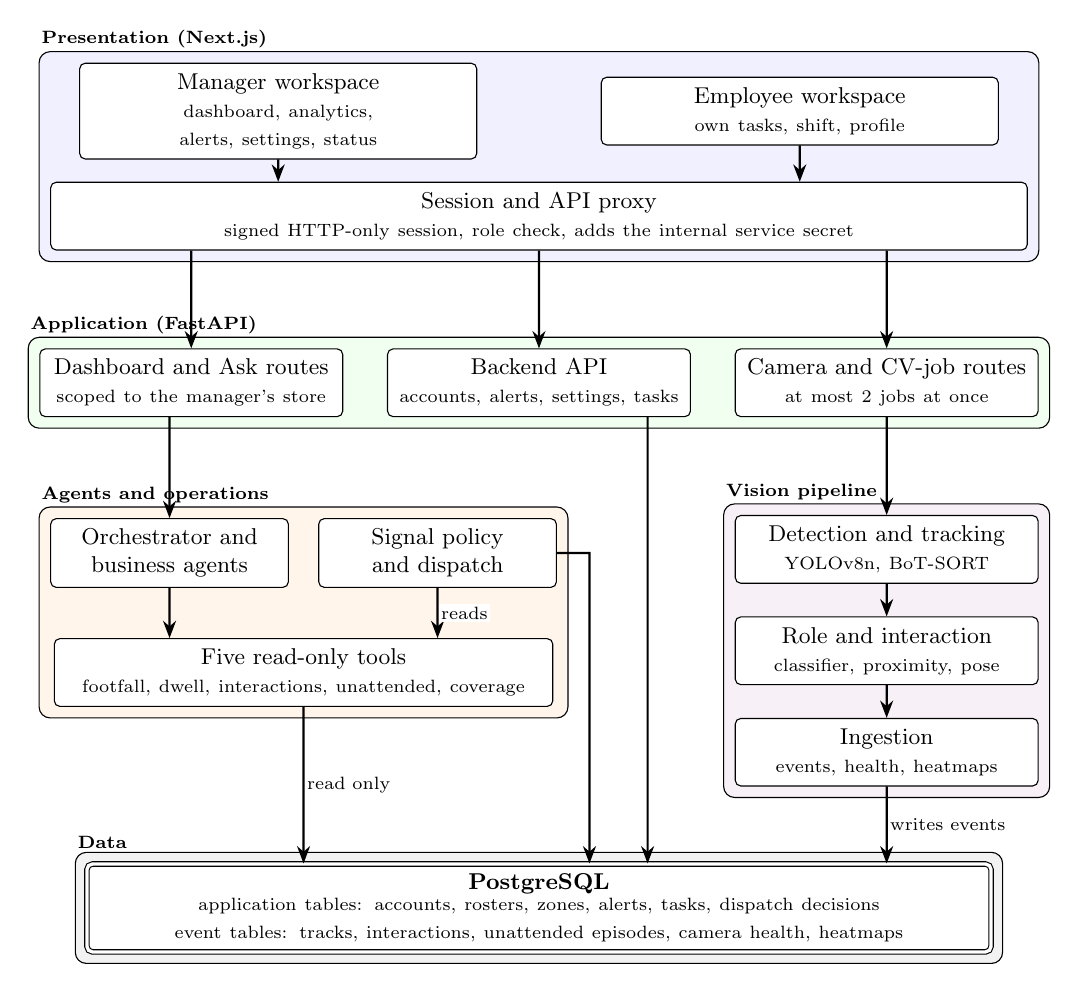
\begin{tikzpicture}[font=\small, scale=0.92, transform shape,
  comp/.style={box, fill=white, text width=#1},
  comp/.default=3.5cm,
  lay/.style={draw, rounded corners=4pt, fill=#1, inner sep=4pt},
  dl/.style={font=\scriptsize, fill=white, inner sep=1pt}]
% presentation
\node[comp=5.2cm] (mgrui) at (3.4,0) {Manager workspace\\\scriptsize dashboard, analytics, alerts, settings, status};
\node[comp=5.2cm] (empui) at (10.6,0) {Employee workspace\\\scriptsize own tasks, shift, profile};
\node[comp=13.2cm] (proxy) at (7.0,-1.45) {Session and API proxy\\\scriptsize signed HTTP-only session, role check, adds the internal service secret};
% application
\node[comp=3.9cm] (dash) at (2.2,-3.75) {Dashboard and Ask routes\\\scriptsize scoped to the manager's store};
\node[comp=3.9cm] (api) at (7.0,-3.75) {Backend API\\\scriptsize accounts, alerts, settings, tasks};
\node[comp=3.9cm] (jobs) at (11.8,-3.75) {Camera and CV-job routes\\\scriptsize at most 2 jobs at once};
% agents and operations
\node[comp=3.0cm] (orch) at (1.9,-6.1) {Orchestrator and business agents};
\node[comp=3.0cm] (signal) at (5.6,-6.1) {Signal policy and dispatch};
\node[comp=6.6cm] (tools) at (3.75,-7.75) {Five read-only tools\\\scriptsize footfall, dwell, interactions, unattended, coverage};
% vision
\node[comp=3.9cm] (det) at (11.8,-6.05) {Detection and tracking\\\scriptsize YOLOv8n, BoT-SORT};
\node[comp=3.9cm] (role) at (11.8,-7.45) {Role and interaction\\\scriptsize classifier, proximity, pose};
\node[comp=3.9cm] (ing) at (11.8,-8.85) {Ingestion\\\scriptsize events, health, heatmaps};
% data
\node[box, double, double distance=1.2pt, text width=12.2cm, fill=white] (db) at (7.0,-11.0) {\textbf{PostgreSQL}\\\scriptsize application tables: accounts, rosters, zones, alerts, tasks, dispatch decisions\\\scriptsize event tables: tracks, interactions, unattended episodes, camera health, heatmaps};
% layers
\begin{scope}[on background layer]
\node[lay=blue!6, fit=(mgrui)(empui)(proxy), label={[font=\scriptsize\bfseries, anchor=south west, inner sep=1pt]north west:Presentation (Next.js)}] {};
\node[lay=green!6, fit=(dash)(api)(jobs), label={[font=\scriptsize\bfseries, anchor=south west, inner sep=1pt]north west:Application (FastAPI)}] {};
\node[lay=orange!8, fit=(orch)(signal)(tools), label={[font=\scriptsize\bfseries, anchor=south west, inner sep=1pt]north west:Agents and operations}] {};
\node[lay=violet!6, fit=(det)(role)(ing), label={[font=\scriptsize\bfseries, anchor=south west, inner sep=1pt]north west:Vision pipeline}] {};
\node[lay=gray!10, fit=(db), label={[font=\scriptsize\bfseries, anchor=south west, inner sep=1pt]north west:Data}] {};
\end{scope}
% flows
\draw[flow] (mgrui) -- (mgrui |- proxy.north);
\draw[flow] (empui) -- (empui |- proxy.north);
\foreach \t in {dash, api, jobs} { \draw[flow] (\t |- proxy.south) -- (\t); }
\draw[flow] (dash.south -| orch) -- (orch);
\draw[flow] (orch) -- (orch |- tools.north);
\draw[flow] (signal) -- node[dl, right] {reads} (signal |- tools.north);
\draw[flow] (jobs) -- (det);
\draw[flow] (det) -- (role);
\draw[flow] (role) -- (ing);
\draw[flow] (tools) -- node[dl, right] {read only} (tools |- db.north);
\draw[flow] (signal.east) -- ++(0.45,0) coordinate (sw) -- (sw |- db.north);
\draw[flow] ([xshift=15mm]api.south) coordinate (aw) -- (aw |- db.north);
\draw[flow] (ing) -- node[dl, right] {writes events} (ing |- db.north);
\end{tikzpicture}
\caption[Layered architecture of RetailPulse]{Layered architecture of RetailPulse. Arrows point from caller to callee. Only the backend API (accounts, alerts, tasks), dispatch (tasks, decisions, alerts) and ingestion (events) write to PostgreSQL; the agents only read.}
\label{fig:architecture}
\end{figure}

\begin{table}[H]
\centering
\caption{Architectural components and responsibilities}\label{tab:components}
\begin{tabular}{P{0.25\textwidth}P{0.42\textwidth}P{0.25\textwidth}}
\toprule
Component & Responsibility & Main source\\
\midrule
Session and API proxy & Signs sessions, checks role, forwards requests with the internal secret and actor identity & \path{frontend/src/app/api/}\\
Backend API & Accounts, invitations, alerts, settings, rosters, tasks and the task event stream & \path{backend/app.py}, \path{store_core.py}\\
Interaction pipeline & Detects, tracks and classifies people; nominates and judges interactions & \path{backend/interaction/}\\
Ingestion & Converts a run's outputs into event rows, camera health and heatmaps & \path{backend/events/ingest.py}\\
Read-only tools & Five typed, scoped analytics readers over the event store & \path{backend/agents/tools/}\\
Orchestrator & Routes a question, runs one business agent, checks every claim & \path{backend/agents/graph.py}\\
Business agents & Customer Behavior and Employee Activity specialists; digest; occupancy & \path{backend/agents/business/}\\
Signal policy & Decides when a window becomes an unattended or unstaffed event & \path{signal_policy.py}\\
Dispatch & Selects an eligible employee, creates the task, prevents duplicates & \path{backend/dispatch.py}\\
\bottomrule
\end{tabular}
\end{table}

\subsection{Agents in the Architecture}
The proposal named seven agent responsibilities. Table~\ref{tab:agent-map} shows where each one is realised. Two are full business agents; the others are realised as deterministic components, because rules are easier to test and explain than a language model wherever the decision is a fixed policy.

\begin{table}[H]
\centering
\caption{Agent responsibilities and their realisation}\label{tab:agent-map}
\begin{tabular}{P{0.27\textwidth}P{0.65\textwidth}}
\toprule
Responsibility & Realisation\\
\midrule
Customer Behavior Agent & Business specialist reading footfall, dwell, interactions and unattended episodes\\
Employee Activity Agent & Business specialist reading staff coverage, interactions and unattended episodes\\
Interaction Agent & The interaction pipeline: proximity nomination plus pose judge\\
Employee Task Assignment Agent & Signal policy plus dispatch service (deterministic eligibility rules)\\
Insight Narration Agent & Digest builder over verified claims, with a narrative number check\\
Query Agent & The orchestrator's question path over the two specialists\\
Orchestrator & LangGraph state graph: route, specialist, ground, repair, finish\\
\bottomrule
\end{tabular}
\end{table}

\section{Vision Pipeline Design}
For every processed frame the pipeline runs the steps in Figure~\ref{fig:pipeline}. A COCO-trained YOLOv8n model detects people and BoT-SORT keeps their track identifiers. A second detector trained on the team's store footage labels each new track as customer or employee during its first second and rechecks it every two seconds, so an identity switch cannot carry an employee label onto a customer. The role decision combines that detector's vote with bib colour and standing still, using the fitted weights adopted after evaluation (Section~\ref{sec:role-weights}).

\begin{figure}[htbp]
\centering
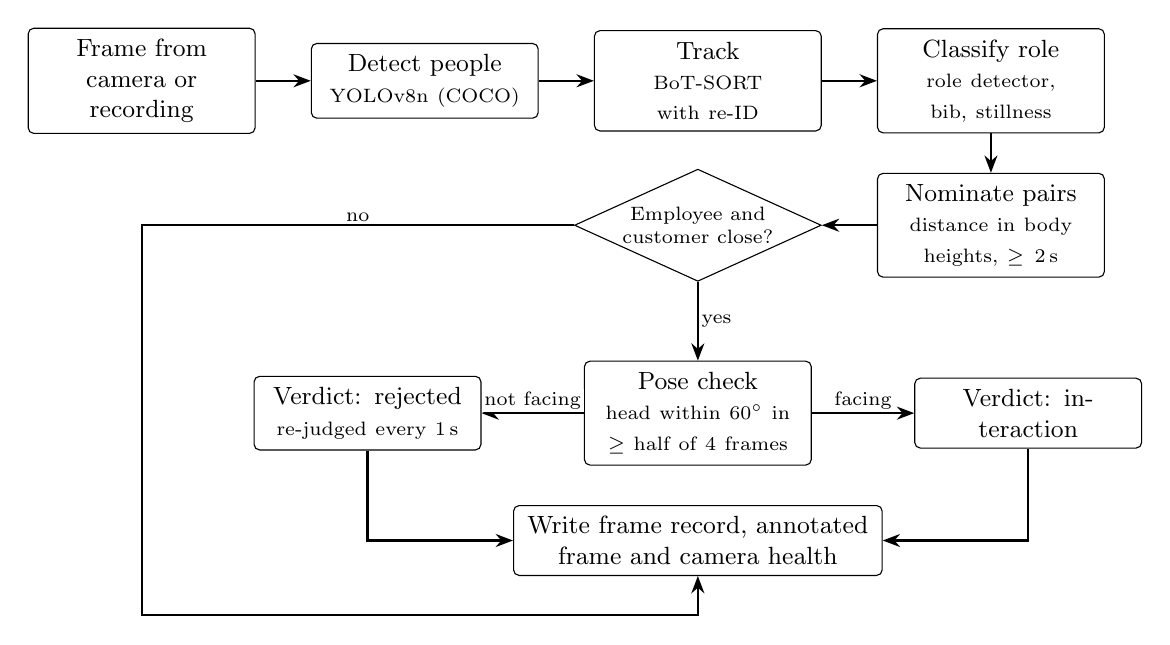
\begin{tikzpicture}[font=\small, node distance=5mm and 7mm,
  pstep/.style={box, text width=2.6cm, fill=white},
  dec/.style={draw, diamond, aspect=2.2, align=center, font=\scriptsize, inner sep=1pt}]
\node[pstep] (in) {Frame from camera or recording};
\node[pstep, right=of in] (detect) {Detect people\\\scriptsize YOLOv8n (COCO)};
\node[pstep, right=of detect] (track) {Track\\\scriptsize BoT-SORT with re-ID};
\node[pstep, right=of track] (roles) {Classify role\\\scriptsize role detector, bib, stillness};
\node[pstep, below=of roles] (prox) {Nominate pairs\\\scriptsize distance in body heights, $\geq 2$\,s};
\node[dec, left=of prox] (cand) {Employee and\\customer close?};
\node[pstep, below=10mm of cand] (judge) {Pose check\\\scriptsize head within $60^\circ$ in $\geq$ half of 4 frames};
\node[pstep, left=of judge, xshift=-6mm] (rej) {Verdict: rejected\\\scriptsize re-judged every 1\,s};
\node[pstep, right=of judge, xshift=6mm] (conf) {Verdict: interaction};
\node[pstep, below=of judge, text width=4.4cm] (out) {Write frame record, annotated frame and camera health};
\draw[flow] (in) -- (detect);
\draw[flow] (detect) -- (track);
\draw[flow] (track) -- (roles);
\draw[flow] (roles) -- (prox);
\draw[flow] (prox) -- (cand);
\draw[flow] (cand) -- node[lbl, right] {yes} (judge);
\draw[flow] (cand.west) -- node[lbl, above] {no} (cand.west -| in.south) -- ([yshift=-5mm]in.south |- out.south) -| (out.south);
\draw[flow] (judge) -- node[lbl, above] {not facing} (rej);
\draw[flow] (judge) -- node[lbl, above] {facing} (conf);
\draw[flow] (rej) |- (out);
\draw[flow] (conf) |- (out);
\end{tikzpicture}
\caption{Per-frame processing in the interaction pipeline}
\label{fig:pipeline}
\end{figure}

Distance is measured in body heights rather than metres: the allowed gap is 1.0 body height between feet, 0.8 between hips and 0.6 between heads, because higher body parts carry less depth information. A pair must stay within that gap for two seconds and must not drift apart faster than walking pace, which removes most pass-bys. If the pose model finds no face or fails, the verdict stays \emph{unverified} rather than being guessed.

\section{Question Answering and Grounding}
A manager's question passes through the orchestration graph in Figure~\ref{fig:graph}. The router either selects one business agent or ends the run as unsupported; questions that mention dispatching, ranking or identifying people are refused before routing. The agent may call only its allowed tools. Every number the agent returns is a \emph{claim} that names a tool call and the path of one metric in its result; the grounding step compares each claim with that metric. A failed claim triggers one repair attempt, and anything that still fails is dropped. The graph never writes to the database.

\begin{figure}[htbp]
\centering
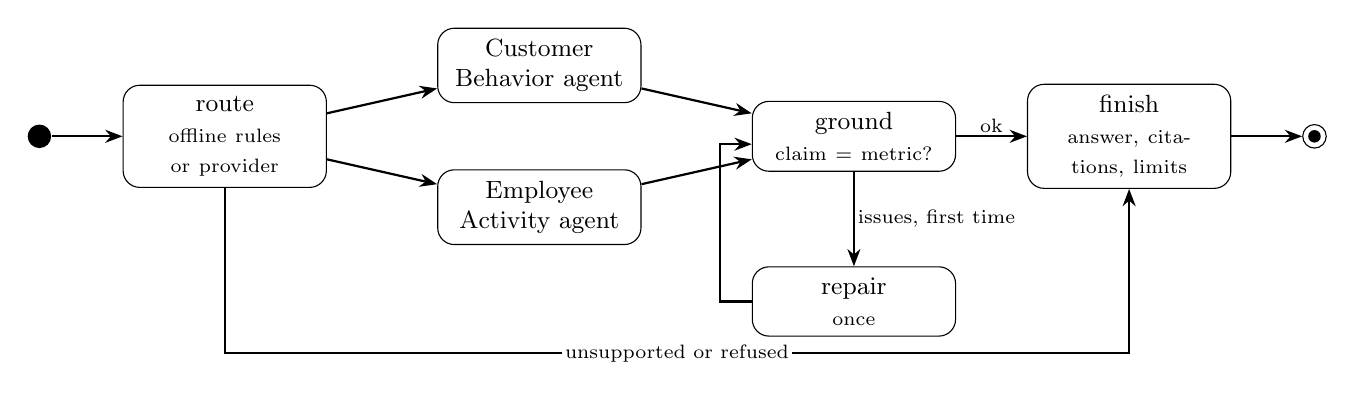
\begin{tikzpicture}[font=\small, node distance=6mm and 9mm,
  st/.style={box, rounded corners=6pt, fill=white, text width=2.3cm}]
\node[circle, fill=black, inner sep=3pt] (s) {};
\node[st, right=of s] (route) {route\\\scriptsize offline rules or provider};
\node[st, right=14mm of route, yshift=9mm] (cb) {Customer Behavior agent};
\node[st, right=14mm of route, yshift=-9mm] (ea) {Employee Activity agent};
\node[st, right=14mm of cb, yshift=-9mm] (ground) {ground\\\scriptsize claim = metric?};
\node[st, below=12mm of ground] (repair) {repair\\\scriptsize once};
\node[st, right=of ground] (finish) {finish\\\scriptsize answer, citations, limits};
\node[circle, draw, inner sep=3pt, right=of finish] (e) {}; \node[circle, fill=black, inner sep=1.6pt] at (e) {};
\draw[flow] (s) -- (route);
\draw[flow] (route) -- (cb);
\draw[flow] (route) -- (ea);
\draw[flow] (route.south) -- ++(0,-2.1) -| node[lbl, pos=0.25] {unsupported or refused} (finish.south);
\draw[flow] (cb) -- (ground);
\draw[flow] (ea) -- (ground);
\draw[flow] (ground) -- node[lbl, right] {issues, first time} (repair);
\draw[flow] (repair.west) -- ++(-4mm,0) |- ([yshift=-1mm]ground.west);
\draw[flow] (ground) -- node[lbl, above] {ok} (finish);
\draw[flow] (finish) -- (e);
\end{tikzpicture}
\caption{Orchestration graph for a manager question}
\label{fig:graph}
\end{figure}

% Design models: domain model, class diagrams, data design, sequence diagrams, state machine, deployment.
\tikzset{
  cls/.style={draw, rectangle split, rectangle split parts=2, rectangle split part align={center,left},
              align=left, font=\scriptsize, fill=white, text width=#1, inner sep=2.5pt,
              execute at begin node={\hyphenpenalty=10000\exhyphenpenalty=10000}},
  cls/.default=2.9cm,
  dcls/.style={draw, rectangle split, rectangle split parts=3, rectangle split part align={center,left,left},
               align=left, font=\scriptsize, fill=white, text width=#1, inner sep=2.5pt,
               execute at begin node={\hyphenpenalty=10000\exhyphenpenalty=10000}},
  dcls/.default=4.6cm,
  rel/.style={thin},
  m/.style={font=\tiny, inner sep=1pt},
  an/.style={font=\tiny\itshape, fill=white, inner sep=1pt},
  compo/.style={thin, {Diamond[fill=black,length=2.6mm,width=1.8mm]}-},
  aggr/.style={thin, {Diamond[open,length=2.6mm,width=1.8mm]}-},
  inherit/.style={thin, -{Triangle[open,length=2.4mm,width=2.4mm]}},
  realize/.style={thin, dashed, -{Triangle[open,length=2.4mm,width=2.4mm]}},
  usedep/.style={thin, dashed, ->},
}

\section{Domain Model}
The domain model (Figure~\ref{fig:domain}) shows the concepts of the problem and how they relate. It contains only real-world concepts and their attributes: software components such as agents, the orchestrator or the database do not appear, and no operations are shown.

\begin{landscape}
\begin{figure}[p]
\centering
\begin{tikzpicture}[scale=0.95, transform shape]
% row 1
\node[cls] (health) at (0,0) {\textbf{CameraHealth}\nodepart{second}minute\\frameRate\\unknownRoleShare\\frozenOrDark};
\node[cls] (camera) at (4.6,0) {\textbf{Camera}\nodepart{second}name\\role\\source};
\node[cls] (store) at (9.2,0) {\textbf{Store}\nodepart{second}name};
\node[cls] (zone) at (13.8,0) {\textbf{Zone}\nodepart{second}name\\type\\capacity\\minimumStaff};
\node[cls] (roster) at (18.4,0) {\textbf{RosterEntry}\nodepart{second}shift\\available};
% row 2
\node[cls] (run) at (4.6,-3.4) {\textbf{AnalysisRun}\nodepart{second}startedAt\\source};
\node[cls=3.5cm] (user) at (18.4,-3.4) {\textbf{StaffMember}\nodepart{second}name\\email\\role (Manager \textbar\ Employee)\\active};
% row 3
\node[cls] (inter) at (0,-6.8) {\textbf{Interaction}\nodepart{second}start\\end\\verdict};
\node[cls] (track) at (4.6,-6.8) {\textbf{Track}\nodepart{second}role\\roleScore\\firstSeen\\lastSeen};
\node[cls] (unatt) at (9.2,-6.8) {\textbf{UnattendedEpisode}\nodepart{second}waitedSeconds\\helped};
\node[cls] (event) at (13.8,-6.8) {\textbf{StaffingEvent}\nodepart{second}type\\window\\severity};
% row 4
\node[cls] (alert) at (9.2,-10.2) {\textbf{Alert}\nodepart{second}category\\severity\\status};
\node[cls] (decision) at (13.8,-10.2) {\textbf{DispatchDecision}\nodepart{second}outcome\\reason};
\node[cls] (task) at (18.4,-10.2) {\textbf{Task}\nodepart{second}instruction\\state\\acknowledgedAfter};

% associations: label in the middle, multiplicities near the ends
\draw[rel] (health) -- node[an, above] {reports on} node[m, below, pos=0.12] {0..*} node[m, below, pos=0.88] {1} (camera);
\draw[rel] (camera) -- node[an, above] {belongs to} node[m, below, pos=0.12] {1..*} node[m, below, pos=0.88] {1} (store);
\draw[rel] (store) -- node[an, above] {has} node[m, below, pos=0.12] {1} node[m, below, pos=0.88] {1..*} (zone);
\draw[rel] (zone) -- node[an, above] {staffed by} node[m, below, pos=0.12] {0..1} node[m, below, pos=0.88] {0..*} (roster);
\draw[rel] ([xshift=6mm]camera.south) -- ++(0,-0.7) -| node[an, pos=0.25] {watches} node[m, right, pos=0.92] {1} ([xshift=-6mm]zone.south)
  node[m, left] at ([xshift=6mm,yshift=-2mm]camera.south) {0..*};
\draw[rel] ([xshift=-6mm]camera.south) -- node[an, left] {produces} node[m, left, pos=0.15] {1} node[m, left, pos=0.85] {0..*} ([xshift=-6mm]run.north);
\draw[rel] (roster) -- node[an, right] {for} node[m, right, pos=0.15] {0..*} node[m, right, pos=0.85] {1} (user);
\draw[rel] (store.north) -- ++(0,0.7) -| node[an, pos=0.25] {employs} node[m, left, pos=0.97] {1..*} ([xshift=2.4cm]user.east) -- (user.east)
  node[m, right] at ([yshift=2mm]store.north) {1};
\draw[rel] (run) -- node[an, left] {contains} node[m, left, pos=0.15] {1} node[m, left, pos=0.85] {0..*} (track);
\draw[rel] ([yshift=3mm]track.west) -- node[an, above] {employee} node[m, below, pos=0.15] {1} node[m, below, pos=0.85] {0..*} ([yshift=3mm]inter.east);
\draw[rel] ([yshift=-3mm]track.west) -- node[an, below] {customer} node[m, below, pos=0.15] {1} node[m, below, pos=0.85] {0..*} ([yshift=-3mm]inter.east);
\draw[rel] (track) -- node[an, above] {waits as} node[m, below, pos=0.12] {1} node[m, below, pos=0.88] {0..1} (unatt);
\draw[rel] (unatt) -- node[an, above] {triggers} node[m, below, pos=0.12] {1..*} node[m, below, pos=0.88] {0..1} (event);
\draw[rel] ([xshift=6mm]zone.south) -- node[an, right] {concerns} node[m, right, pos=0.1] {1} node[m, right, pos=0.9] {0..*} ([xshift=6mm]event.north);
\draw[rel] (event) -- node[an, right] {decided by} node[m, right, pos=0.15] {1} node[m, right, pos=0.85] {1} (decision);
\draw[rel] (decision) -- node[an, above] {raises} node[m, below, pos=0.12] {1} node[m, below, pos=0.88] {0..1} (alert);
\draw[rel] (decision) -- node[an, above] {creates} node[m, below, pos=0.12] {1} node[m, below, pos=0.88] {0..1} (task);
\draw[rel] (task) -- node[an, right] {assigned to} node[m, right, pos=0.12] {0..*} node[m, right, pos=0.88] {1} (user);
\draw[rel] (alert.south) -- ++(0,-0.7) -| node[an, pos=0.25] {resolved by} node[m, left, pos=0.97] {0..1} ([xshift=2.9cm,yshift=-4mm]user.east) -- ([yshift=-4mm]user.east)
  node[m, right] at ([yshift=-2mm]alert.south) {0..*};
\end{tikzpicture}
\caption{Domain model}
\label{fig:domain}
\end{figure}
\end{landscape}

\section{Class Diagrams}
The class diagrams show the main design classes with their real names, typed attributes and operations with return types. Figure~\ref{fig:class-vision} covers the vision pipeline and Figure~\ref{fig:class-agents} the agent and operations layer. Helper classes and private members are omitted.

\begin{figure}[htbp]
\centering
\begin{tikzpicture}[scale=0.9, transform shape]
% the pipeline and its configuration (left)
\node[dcls=4.3cm] (cfg) at (0,3.3) {\textbf{InteractionConfig}
  \nodepart{second}min\_interaction\_seconds: float = 2.0\\facing\_angle\_degrees: float = 60\\min\_facing\_fraction: float = 0.5\\role\_weights: dict[str, float]
  \nodepart{third}from\_json(path: Path): InteractionConfig};
\node[dcls=4.3cm] (pipe) at (0,-0.6) {\textbf{InteractionPipeline}
  \nodepart{second}config: InteractionConfig\\judge: PoseJudge \textbar\ None
  \nodepart{third}process\_frame(frame: ndarray,\\\quad timestamp: float): dict\\verdict(event: InteractionEvent): str};
% the four parts (middle column)
\node[dcls=4.5cm] (tracker) at (6.1,3.3) {\textbf{ByteTrackPersonTracker}
  \nodepart{second}tracker: str = "botsort\_reid.yaml"
  \nodepart{third}detect\_and\_track(frame: ndarray,\\\quad timestamp: float): list[dict]};
\node[dcls=4.5cm] (roles) at (6.1,1.05) {\textbf{RoleClassifier}
  \nodepart{second}agent: CustEmpClassifier
  \nodepart{third}classify(frame: ndarray, bbox: tuple,\\\quad track\_id: int, timestamp: float):\\\quad tuple[str, float, dict]};
\node[dcls=4.5cm] (eng) at (6.1,-1.45) {\textbf{EngagementDetector}
  \nodepart{second}config: InteractionConfig
  \nodepart{third}update(people: list[TrackedPerson],\\\quad timestamp: float, frame\_height: int):\\\quad list[InteractionEvent]};
\node[dcls=4.5cm] (judge) at (6.1,-3.95) {\textbf{PoseJudge}
  \nodepart{second}facing\_angle: float\\min\_facing\_fraction: float
  \nodepart{third}classify\_interaction(frames: list,\\\quad boxes: list): JudgeResult};
% results and helpers (right column)
\node[dcls=3.7cm] (cec) at (11.6,1.05) {\textbf{CustEmpClassifier}
  \nodepart{second}weights: dict[str, float]\\threshold: float
  \nodepart{third}decide(factors: dict):\\\quad tuple[str, float, dict]};
\node[dcls=3.7cm] (event) at (11.6,-1.45) {\textbf{InteractionEvent}
  \nodepart{second}employee\_track\_id: int\\customer\_track\_id: int\\started\_at: float\\distance\_body\_heights: float\\active: bool
  \nodepart{third}};
\node[dcls=3.7cm] (jr) at (11.6,-3.95) {\textbf{JudgeResult}
  \nodepart{second}label: str\\confidence: float
  \nodepart{third}};
\draw[usedep] (pipe) -- node[an, right] {configured by} (cfg);
% composition: one diamond at the whole, a bus to each part
\draw[compo] (pipe.east) -- ++(0.8,0) coordinate (bus);
\draw[thin] (bus |- tracker) -- (bus |- judge);
\draw[thin] (bus |- tracker) -- node[m, above, pos=0.8] {1} (tracker.west);
\draw[thin] (bus |- roles) -- node[m, above, pos=0.8] {1} (roles.west);
\draw[thin] (bus |- eng) -- node[m, above, pos=0.8] {1} (eng.west);
\draw[thin] (bus |- judge) -- node[m, above, pos=0.8] {0..1} (judge.west);
\draw[compo] (roles) -- node[m, above, pos=0.8] {1} (cec);
\draw[usedep] (eng) -- node[an, above] {creates} (event);
\draw[usedep] (judge) -- node[an, above] {returns} (jr);
\end{tikzpicture}
\caption{Class diagram: vision pipeline}
\label{fig:class-vision}
\end{figure}

\begin{figure}[htbp]
\centering
\begin{tikzpicture}[scale=0.9, transform shape]
% question path (left and middle)
\node[dcls=4.4cm] (svc) at (0,0) {\textbf{AnalyticsService}
  \nodepart{second}traces: MemoryTraceStore
  \nodepart{third}ask(request: AskRequest,\\\quad scope: TrustedAccessScope): GraphRun\\get\_run(run\_id: str,\\\quad scope: TrustedAccessScope): GraphRun};
\node[dcls=3.9cm] (spec) at (0,-3.7) {\textbf{SpecialistRegistration}
  \nodepart{second}handler: Callable\\allowed\_tools: frozenset[str]\\development\_stub: bool
  \nodepart{third}};
\node[dcls=4.4cm] (reg) at (5.8,0) {\textbf{ScopedToolRegistry}
  \nodepart{second}scope: TrustedAccessScope
  \nodepart{third}invoke(name: str, arguments: dict):\\\quad ToolResult\\input\_schemas(): dict};
\node[dcls=4.4cm] (ea) at (5.8,-3.7) {\textbf{EventAnalytics}
  \nodepart{second}dsn: str\\synthetic: bool
  \nodepart{third}get\_footfall(scope, request): FootfallResult\\get\_zone\_dwell(scope, request):\\\quad ZoneDwellResult\\get\_interactions(scope, request):\\\quad InteractionsResult};
\node[dcls=4.4cm] (pg) at (5.8,-7.6) {\textbf{PostgresAnalyticsTools}
  \nodepart{second}contexts: tuple[ObservationContext]
  \nodepart{third}get\_unattended(scope, request):\\\quad UnattendedResult\\get\_coverage(scope, request):\\\quad CoverageResult};
% operations path (right and bottom)
\node[dcls=4.1cm] (pol) at (11.4,0) {\textbf{SignalPolicy}
  \nodepart{second}min\_wait\_s: float = 180\\high\_wait\_s: float = 360\\min\_staffed\_ratio: float = 0.25\\max\_unknown\_share: float = 0.2
  \nodepart{third}};
\node[dcls=4.1cm] (dec) at (11.4,-3.7) {\textbf{SignalDecision}
  \nodepart{second}event\_type: str\\zone\_id: str\\reason: ReasonCode\\event: OperationalEvent \textbar\ None
  \nodepart{third}};
\node[dcls=4.1cm] (oe) at (11.4,-7.6) {\textbf{OperationalEvent}
  \nodepart{second}event\_id: str\\idempotency\_key: str\\zone\_id: str\\event\_type: str\\severity: str
  \nodepart{third}};
\node[dcls=4.1cm] (ad) at (11.4,-11.3) {\textbf{OperationalDispatchAdapter}
  \nodepart{second}handler: DispatchHandler
  \nodepart{third}handle(event: OperationalEvent,\\\quad scope: TrustedOperationalScope):\\\quad DispatchReceipt};
\node[dcls=4.4cm] (dh) at (5.8,-11.3) {\guillemotleft interface\guillemotright\\\textbf{DispatchHandler}
  \nodepart{second}
  \nodepart{third}\_\_call\_\_(event: OperationalEvent,\\\quad scope: TrustedOperationalScope):\\\quad DispatchOutcome};
\node[dcls=4.4cm] (disp) at (0,-11.3) {\guillemotleft module\guillemotright\\\textbf{dispatch}
  \nodepart{second}ACTIVE\_TASK\_STATES: tuple[str]
  \nodepart{third}handle\_event(conn, body: dict): dict\\select\_dispatch\_employee(conn,\\\quad target\_zone\_id: str): Row \textbar\ None\\make\_dispatch\_handler(dsn: str):\\\quad DispatchHandler};
\draw[usedep] (svc) -- node[an, above] {\guillemotleft create\guillemotright} (reg);
\draw[aggr] (svc) -- node[m, left, pos=0.85] {0..2} (spec);
\draw[aggr] (reg) -- node[m, right, pos=0.85] {1} (ea);
\draw[inherit] (pg) -- (ea);
\draw[usedep] (dec) -- node[an, right] {\guillemotleft use\guillemotright\ thresholds} (pol);
\draw[usedep] (dec.west) -- ++(-0.5,0) |- node[an, pos=0.75] {\guillemotleft use\guillemotright\ reads tools} (reg.east);
\draw[aggr] (dec) -- node[m, right, pos=0.85] {0..1} (oe);
\draw[usedep] (ad) -- node[an, right] {handles} (oe);
\draw[aggr] (ad) -- node[m, above, pos=0.8] {1} (dh);
\draw[usedep] (disp) -- node[an, above] {\guillemotleft create\guillemotright} (dh);
\end{tikzpicture}
\caption{Class diagram: agents and operations}
\label{fig:class-agents}
\end{figure}

\section{Data Design}
All persistent data is in one PostgreSQL database with two groups of tables. The \emph{application tables} (Figure~\ref{fig:erd}) hold accounts, store configuration and the operational record of every dispatch decision. The \emph{event tables} (Table~\ref{tab:event-tables}) hold what the cameras observed; they share one set of common columns and are linked by run, camera and track identifiers rather than foreign keys, because a run is always written and replaced as a whole.

\begin{figure}[htbp]
\centering
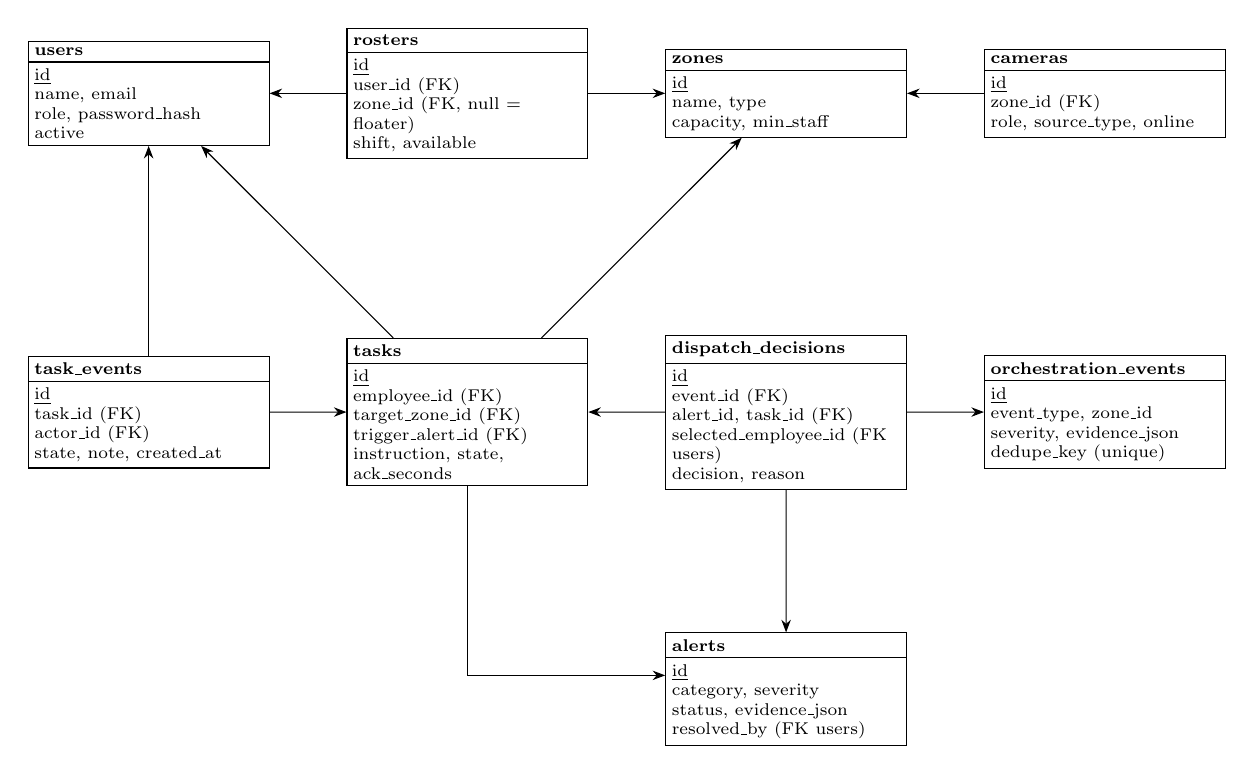
\begin{tikzpicture}[scale=0.88, transform shape,
  tbl/.style={draw, rectangle split, rectangle split parts=2, rectangle split part align={center,left},
              align=left, font=\scriptsize, fill=white, text width=3.3cm, inner sep=2.5pt,
              rectangle split part fill={gray!15,white}},
  fk/.style={thin, -{Stealth[length=1.6mm]}},
  m/.style={font=\tiny, inner sep=1pt}]
\node[tbl] (users) at (0,0) {\textbf{users}\nodepart{second}\underline{id}\\name, email\\role, password\_hash\\active};
\node[tbl] (rosters) at (4.6,0) {\textbf{rosters}\nodepart{second}\underline{id}\\user\_id (FK)\\zone\_id (FK, null = floater)\\shift, available};
\node[tbl] (zones) at (9.2,0) {\textbf{zones}\nodepart{second}\underline{id}\\name, type\\capacity, min\_staff};
\node[tbl] (cameras) at (13.8,0) {\textbf{cameras}\nodepart{second}\underline{id}\\zone\_id (FK)\\role, source\_type, online};
\node[tbl] (events) at (13.8,-4.6) {\textbf{orchestration\_events}\nodepart{second}\underline{id}\\event\_type, zone\_id\\severity, evidence\_json\\dedupe\_key (unique)};
\node[tbl] (dd) at (9.2,-4.6) {\textbf{dispatch\_decisions}\nodepart{second}\underline{id}\\event\_id (FK)\\alert\_id, task\_id (FK)\\selected\_employee\_id (FK users)\\decision, reason};
\node[tbl] (tasks) at (4.6,-4.6) {\textbf{tasks}\nodepart{second}\underline{id}\\employee\_id (FK)\\target\_zone\_id (FK)\\trigger\_alert\_id (FK)\\instruction, state, ack\_seconds};
\node[tbl] (tev) at (0,-4.6) {\textbf{task\_events}\nodepart{second}\underline{id}\\task\_id (FK)\\actor\_id (FK)\\state, note, created\_at};
\node[tbl] (alerts) at (9.2,-8.6) {\textbf{alerts}\nodepart{second}\underline{id}\\category, severity\\status, evidence\_json\\resolved\_by (FK users)};
% foreign keys point from the referencing table to the referenced table
\draw[fk] (rosters) -- (users);
\draw[fk] (rosters) -- (zones);
\draw[fk] (cameras) -- (zones);
\draw[fk] (tasks) -- (users);
\draw[fk] (tasks) -- (zones);
\draw[fk] (tev) -- (tasks);
\draw[fk] (tev) -- (users);
\draw[fk] (dd) -- (events);
\draw[fk] (dd) -- (tasks);
\draw[fk] (dd) -- (alerts);
\draw[fk] (tasks.south) |- ([yshift=2mm]alerts.west);
\end{tikzpicture}
\caption[Application tables]{Application tables. Arrows run from a foreign key to the table it references; the two references to \texttt{users} from \texttt{alerts} and \texttt{dispatch\_decisions} are named in the column instead of drawn. Only key columns are shown.}
\label{fig:erd}
\end{figure}

\begin{table}[H]
\centering
\caption{Event tables (common columns: event\_id, run\_id, store\_id, camera\_id, zone\_id, ts\_start, ts\_end)}\label{tab:event-tables}
\begin{tabular}{P{0.24\textwidth}P{0.68\textwidth}}
\toprule
Table & Additional content\\
\midrule
tracks & track\_id, role, employee\_score, frames\_observed\\
role\_decisions & track\_id, role, frames\\
interactions & employee and customer track\_id, duration\_s, verdict (interaction, no\_interaction, unverified)\\
unattended\_episodes & customer\_track\_id, waited\_s, helped\\
zone\_dwell / cell\_dwell & track\_id, role, dwell\_s (per zone or per registered map cell)\\
footfall & track\_id, direction (in or out)\\
queue\_samples & queue\_length, est\_wait\_s\\
pipeline\_health & fps, mean\_confidence, unknown\_role\_share, id\_churn, frozen\_or\_dark (one row per camera per minute)\\
heatmaps & cols, rows, cells (one grid per camera per hour)\\
\bottomrule
\end{tabular}
\end{table}

Two rules protect the data. Every event row must pass the contract check \texttt{validate()}: the common identifiers are non-empty and no row ends before it starts. And \texttt{dedupe\_key} on \texttt{orchestration\_events} is unique, so the same staffing event can never be inserted twice; the insert uses \texttt{ON CONFLICT DO NOTHING} and the handler then returns the earlier decision.

\section{Interaction Design}
\tikzset{
  life/.style={draw, fill=white, font=\scriptsize, align=center, minimum height=7mm, inner sep=2pt, text width=1.9cm},
  msg/.style={->, thin, >={Stealth[length=1.8mm]}},
  ret/.style={->, thin, dashed, >={Stealth[length=1.8mm]}},
  ml/.style={font=\tiny, above, inner sep=1pt, align=center},
}
\subsection{Staffing Dispatch}
Figure~\ref{fig:seq-dispatch} shows how a closed observation window becomes a task (UC-12). The operations cycle runs after each window for every configured zone. The policy reads three tool results; only if a customer waited past the threshold and the camera could see enough of the window does it emit an event. The dispatch handler then works inside one transaction: it records the event, which fails harmlessly for a duplicate, selects an eligible employee, and writes the alert, task, task event and decision together.

\begin{figure}[htbp]
\centering
\begin{tikzpicture}[scale=0.86, transform shape]
\foreach \x/\n/\t in {0/cyc/Operations\\cycle, 2.45/pol/Signal policy, 4.9/tools/Read-only\\tools, 7.35/ad/Dispatch\\adapter, 9.8/hd/Dispatch\\handler, 12.25/db/PostgreSQL, 14.7/emp/Employee\\page} {
  \node[life] (\n) at (\x,0) {\t};
  \draw[dashed, gray] (\n.south) -- (\x,-13.6);
}
\draw[msg] (0,-1.0) -- node[ml] {evaluate\_zone(zone, window)} (2.45,-1.0);
\draw[msg] (2.45,-1.6) -- node[ml] {get\_unattended, get\_zone\_dwell,\\get\_coverage} (4.9,-1.6);
\draw[msg] (4.9,-2.2) -- node[ml] {read-only SELECT} (12.25,-2.2);
\draw[ret] (12.25,-2.7) -- node[ml] {rows} (4.9,-2.7);
\draw[ret] (4.9,-3.2) -- node[ml] {typed results with evidence} (2.45,-3.2);
\node[draw, font=\tiny, fill=yellow!10, align=left, text width=2.2cm] at (1.2,-4.2) {wait $\geq$ min\_wait\_s,\\unknown share $\leq$ max};
\draw[ret] (2.45,-5.0) -- node[ml] {SignalDecision(event)} (0,-5.0);
\draw[msg] (0,-5.6) -- node[ml] {handle(event, scope)} (7.35,-5.6);
\draw[msg] (7.35,-6.2) -- node[ml] {handler(event, scope)} (9.8,-6.2);
\draw[msg] (9.8,-6.8) -- node[ml] {INSERT event ON CONFLICT (dedupe\_key) DO NOTHING} (12.25,-6.8);
% alt fragment
\draw (8.9,-7.3) rectangle (13.3,-12.0);
\node[draw, font=\tiny\bfseries, anchor=north west, inner sep=1.5pt] at (8.9,-7.3) {alt};
\node[font=\tiny, anchor=north west] at (9.5,-7.35) {[key already stored]};
\draw[ret] (12.25,-8.0) -- node[ml] {earlier decision (duplicate)} (9.8,-8.0);
\draw[dashed] (8.9,-8.4) -- (13.3,-8.4);
\node[font=\tiny, anchor=north west] at (9.0,-8.45) {[new event]};
\draw[msg] (9.8,-9.1) -- node[ml] {select eligible employee} (12.25,-9.1);
\draw[ret] (12.25,-9.6) -- node[ml] {employee or none} (9.8,-9.6);
\draw[msg] (9.8,-10.3) -- node[ml] {INSERT alert, task, task\_event,\\dispatch\_decision; COMMIT} (12.25,-10.3);
\node[font=\tiny, align=left, anchor=west] at (9.85,-11.3) {no employee: alert and\\decision only, no task};
\draw[ret] (9.8,-12.6) -- node[ml] {DispatchOutcome} (7.35,-12.6);
\draw[ret] (7.35,-13.0) -- node[ml] {DispatchReceipt} (0,-13.0);
\draw[msg] (12.25,-13.4) -- node[ml] {task stream event} (14.7,-13.4);
\end{tikzpicture}
\caption{Sequence diagram: unattended customer to staffing task}
\label{fig:seq-dispatch}
\end{figure}

\subsection{Manager Question}
Figure~\ref{fig:seq-ask} shows UC-04. The web tier never forwards a question without a valid manager session, and the Ask route rejects the question if the manager has already asked ten in the current minute. The orchestrator works only through the scoped registry, which is bound to the manager's store.

\begin{figure}[htbp]
\centering
\begin{tikzpicture}[scale=0.86, transform shape]
\foreach \x/\n/\t in {0/mgr/Manager, 2.45/web/Web tier\\and proxy, 4.9/ask/Ask route, 7.35/orc/Orchestrator, 9.8/agent/Business\\agent, 12.25/tl/Read-only\\tools, 14.7/pg/PostgreSQL} {
  \node[life] (\n) at (\x,0) {\t};
  \draw[dashed, gray] (\n.south) -- (\x,-8.4);
}
\draw[msg] (0,-1.0) -- node[ml] {question} (2.45,-1.0);
\draw[msg] (2.45,-1.6) -- node[ml] {question, interval, filters,\\actor + internal secret} (4.9,-1.6);
\node[draw, font=\tiny, fill=yellow!10, align=left, text width=2.0cm, anchor=north west] at (5.05,-2.05) {manager of this store?\\fewer than 10 per minute?};
\draw[msg] (4.9,-3.25) -- node[ml] {ask(request, scope)} (7.35,-3.25);
\draw[msg] (7.35,-3.7) -- node[ml] {route, then run} (9.8,-3.7);
\draw[msg] (9.8,-4.3) -- node[ml] {invoke(tool, arguments)} (12.25,-4.3);
\draw[msg] (12.25,-4.9) -- node[ml] {read-only query} (14.7,-4.9);
\draw[ret] (14.7,-5.3) -- node[ml] {rows} (12.25,-5.3);
\draw[ret] (12.25,-5.7) -- node[ml] {result with evidence} (9.8,-5.7);
\draw[ret] (9.8,-6.2) -- node[ml] {draft claims} (7.35,-6.2);
\draw[msg] (7.35,-6.6) arc[start angle=90, end angle=-90, radius=0.25] node[font=\tiny, right, pos=0.5] {ground claims};
\draw[ret] (7.35,-7.4) -- node[ml] {answer, citations, limitations} (4.9,-7.4);
\draw[ret] (4.9,-7.8) -- (2.45,-7.8);
\draw[ret] (2.45,-8.2) -- node[ml] {answer shown on dashboard} (0,-8.2);
\end{tikzpicture}
\caption{Sequence diagram: manager asks an analytics question}
\label{fig:seq-ask}
\end{figure}

\subsection{Task Lifecycle}
A dispatched task is created in the \emph{delivered} state. Figure~\ref{fig:task-states} shows the intended lifecycle. The backend does not yet enforce these transitions: it accepts any of the listed states from the task's owner or a manager and records each change as a task event, so enforcing the order is listed as FYP-2 work. The first acknowledgement also stores the acknowledgement time, which System Status reports.

\begin{figure}[htbp]
\centering
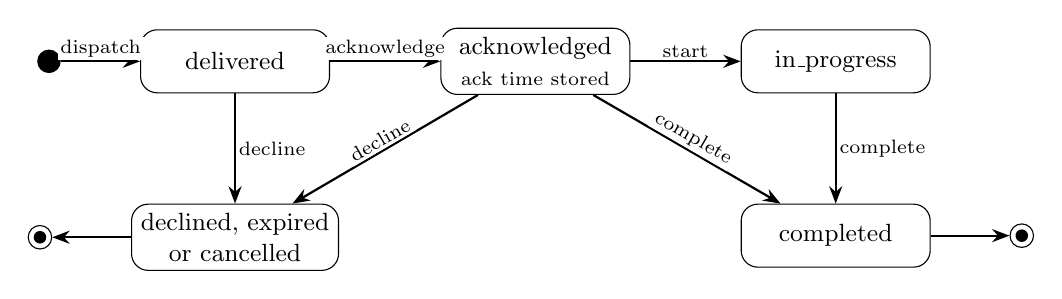
\begin{tikzpicture}[font=\small, node distance=8mm and 14mm,
  state/.style={draw, rounded corners=6pt, minimum width=2.4cm, minimum height=8mm, fill=white, align=center}]
\node[circle, fill=black, inner sep=3pt] (init) {};
\node[state, right=10mm of init] (deliv) {delivered};
\node[state, right=of deliv] (ack) {acknowledged\\\scriptsize ack time stored};
\node[state, right=of ack] (prog) {in\_progress};
\node[state, below=14mm of prog] (done) {completed};
\node[state, below=14mm of deliv] (stop) {declined, expired\\or cancelled};
\node[circle, draw, inner sep=3pt, right=10mm of done] (fin) {}; \node[circle, fill=black, inner sep=1.6pt] at (fin) {};
\node[circle, draw, inner sep=3pt, left=10mm of stop] (fin2) {}; \node[circle, fill=black, inner sep=1.6pt] at (fin2) {};
\draw[flow] (init) -- node[lbl, above] {dispatch} (deliv);
\draw[flow] (deliv) -- node[lbl, above] {acknowledge} (ack);
\draw[flow] (ack) -- node[lbl, above] {start} (prog);
\draw[flow] (prog) -- node[lbl, right] {complete} (done);
\draw[flow] (ack) -- node[lbl, sloped, above] {complete} (done);
\draw[flow] (deliv) -- node[lbl, right] {decline} (stop);
\draw[flow] (ack) -- node[lbl, sloped, above] {decline} (stop);
\draw[flow] (done) -- (fin);
\draw[flow] (stop) -- (fin2);
\end{tikzpicture}
\caption{State machine of a staffing task}
\label{fig:task-states}
\end{figure}

\section{Deployment}
Figure~\ref{fig:deployment} shows the deployment the system is built for. The web tier is deployed on Vercel and the database is a hosted PostgreSQL service (Neon). The Python backend and vision pipeline run on one CPU computer near the cameras, because video should not leave the store. At the time of writing the backend has been run only on team laptops; deploying it is part of the FYP-2 plan (Chapter~\ref{ch:conclusion}).

\begin{figure}[htbp]
\centering
\begin{tikzpicture}[font=\small,
  node3d/.style={draw, fill=white, align=center, inner sep=5pt, font=\scriptsize},
  art/.style={draw, fill=white, align=center, font=\scriptsize, inner sep=3pt, text width=3.2cm},
  conn/.style={thin, <->, >={Stealth[length=1.8mm]}},
  cl/.style={font=\tiny, fill=white, inner sep=1pt, align=center}]
% browser
\node[art] (br) at (0,0) {\guillemotleft artifact\guillemotright\\Web pages (React 19)};
\node[art] (nx) at (6.2,0) {\guillemotleft artifact\guillemotright\\Next.js 15 app,\\session and API proxy};
\node[art] (be) at (6.2,-3.6) {\guillemotleft artifact\guillemotright\\FastAPI backend (Uvicorn):\\API, agents, dispatch};
\node[art] (cv) at (6.2,-5.5) {\guillemotleft artifact\guillemotright\\Vision pipeline jobs:\\YOLOv8n, best\_320, pose};
\node[art] (cam) at (0,-4.55) {\guillemotleft device\guillemotright\\CCTV cameras or\\recorded video};
\node[art] (pg) at (12.2,-3.6) {\guillemotleft database\guillemotright\\PostgreSQL 17};
\begin{scope}[on background layer]
\node[node3d, fill=gray!8, fit=(br), inner sep=8pt, label={[font=\scriptsize]above:\guillemotleft device\guillemotright\ Browser}] (dev) {};
\node[node3d, fill=gray!8, fit=(nx), inner sep=8pt, label={[font=\scriptsize]above:\guillemotleft cloud\guillemotright\ Vercel}] (vc) {};
\node[node3d, fill=gray!8, fit=(be)(cv), inner sep=8pt, label={[font=\scriptsize]below:\guillemotleft device\guillemotright\ Store application host (CPU only)}] (host) {};
\node[node3d, fill=gray!8, fit=(pg), inner sep=8pt, label={[font=\scriptsize]above:\guillemotleft cloud\guillemotright\ Neon}] (neon) {};
\end{scope}
% external
\node[art] (ext) at (12.2,0) {\guillemotleft service\guillemotright\\Hugging Face router,\\ElevenLabs (optional)};
\draw[conn] (dev) -- node[cl, above] {HTTPS} (vc);
\draw[conn] (vc) -- node[cl, left, pos=0.35] {HTTPS, internal secret,\\actor headers} (vc |- host.north);
\draw[conn] (host.east |- pg) -- node[cl, above] {TLS (sslmode=require)} (neon);
\draw[conn] (host.north east) -- node[cl, sloped, above] {HTTPS} (ext);
\draw[conn] (cam) -- node[cl, above] {stream / files} (host.west |- cam);
\end{tikzpicture}
\caption{Deployment diagram}
\label{fig:deployment}
\end{figure}



\chapter{Implementation}
\label{ch:impl}

The system was built in two iterations. Iteration~1 ran from the start of the project to the mid evaluation on 21 October 2026 and produced the vision prototype and the first web application. Iteration~2 ran from the mid evaluation to the submission of this report and turned the prototype into a connected system: a shared database, the event store, the agents, dispatch, the dashboard binding and security hardening. All code is in the repository \path{muhammad-moiz-ansari/retail-store-analysis}; this report describes the \path{fyp2-moiz} branch at commit \texttt{c8ff409} (26 November 2026).

\section{Technology Stack}
\begin{table}[H]
\centering
\caption{Technology stack}\label{tab:stack}
\begin{tabular}{P{0.2\textwidth}P{0.42\textwidth}P{0.3\textwidth}}
\toprule
Layer & Technology & Why\\
\midrule
Vision & Python 3.11, Ultralytics YOLOv8n and YOLOv8n-pose, OpenVINO, BoT-SORT, OpenCV & Small models that run on a CPU; OpenVINO speeds up CPU inference\\
Backend & FastAPI on Uvicorn, Pydantic contracts & Typed request and result models that reject malformed data\\
Agents & LangGraph state graph, five typed read-only tools & Explicit, testable control flow; no free database access\\
Database & PostgreSQL 17 (Neon for the hosted instance), psycopg 3 & One database for application, event and identity data\\
Web & Next.js 15, React 19, TypeScript, Recharts & Server-side session handling and a proxy that keeps secrets off the browser\\
Testing & pytest, Node test runner, GitHub Actions & Three CI jobs on every push\\
Optional services & Hugging Face inference router, ElevenLabs & Question routing and spoken task instructions\\
\bottomrule
\end{tabular}
\end{table}

\section{Iteration 1: Vision Prototype and Web Application}
Iteration~1 established the pieces later work builds on.
\begin{itemize}
\item \textbf{Dataset.} The team recorded its own footage because retailers would not share theirs; the supervisor accepted the resulting 70-video dataset on 12 October 2026. A role detector (\path{best.pt}) was trained on customer and employee classes.
\item \textbf{Interaction pipeline.} Body-height-normalised proximity nominated employee--customer pairs, a pass-by filter rejected people walking past, and a YOLO pose judge checked whether heads faced each other. On the one labelled clip available then, the judge removed the only false positive.
\item \textbf{Web application.} A Next.js application with manager and employee pages, signed session cookies and an internal secret on backend calls.
\item \textbf{Descoped floor prototype.} A calibrated floor-distance prototype projected foot points into metres. The moving-camera footage produced almost no valid projections, so it was descoped in favour of body-height distance.
\end{itemize}
The mid evaluation found the report's figures and requirements incorrect. Iteration~2 therefore included rebuilding both, which this report presents.

\section{Iteration 2: From Prototype to Connected System}

\subsection{Model Consolidation}
Tests on corridor footage showed that the store-trained role detector missed clearly visible people (it found 53--56 of the 140 people that the COCO model found), because it had only seen the team's store. The pipeline now uses the COCO YOLOv8n model to find and track everyone, and runs the role detector only to label each new track during its first second, rechecking every two seconds. When every visible track already has a fresh label, the role detector does not run at all, which saves CPU time.

\subsection{Labelling and Evaluation Tooling}
Twenty-five clips were labelled in CVAT with interaction intervals, pass-bys and reviewed person roles, and imported with \path{cvat_import.py}. A benchmark command scores detector, interaction, role, tracking and speed results; a confidence command adds bootstrap intervals; and a refit command fits role weights with leave-one-clip-out validation. Chapter~\ref{ch:cveval} reports the results.

\subsection{Event Store and PostgreSQL}
Every run is converted by \path{backend/events/ingest.py} into the ten event tables of Table~\ref{tab:event-tables}. Ingestion derives unattended episodes (a customer who waits past the store's threshold without a \emph{confirmed} interaction), per-minute camera health, hourly heatmaps and, for an entrance camera, directional footfall with hysteresis so that a person hovering on the line is counted once. A synthetic fixture day\label{sec:fixture} with planted patterns (an evening rush, an understaffed aisle and a blocked camera) lets every later layer be tested before real footage is stored.

On 11 November 2026 the application moved from SQLite to PostgreSQL, so that accounts, events and camera identities share one database. Analytics reads run in read-only, repeatable-read transactions, and legacy SQLite data can be imported in one transaction with identifiers and password hashes preserved. Ingestion is currently a command run after a job; triggering it automatically when a web-started job finishes is FYP-2 work.

\subsection{Agent Layer}
The agent layer was built in four steps:
\begin{enumerate}
\item \textbf{Typed contracts and five read-only tools} (footfall, zone dwell, interactions, unattended episodes, coverage). Each result carries its time window, filters, evidence references and limitations, and returns \emph{unavailable} rather than zero when its source is missing.
\item \textbf{A scoped registry} that binds tools to the caller's store and allowed runs, cameras and zones, and rejects any attempt to override them in the tool arguments.
\item \textbf{The orchestration graph} (Figure~\ref{fig:graph}) with routing, grounding, one repair and development traces. The router can optionally ask a language model which agent should answer; the model sees only the question and cannot choose tools or supply figures.
\item \textbf{Two business agents.} The Customer Behavior agent answers questions about traffic, dwell, interactions and waiting customers; the Employee Activity agent answers questions about staff coverage and assistance. Both are registered as real agents, not development stubs, and build their answers only from claims that point at tool metrics.
\end{enumerate}
On top of these, the \emph{Insight Narration} digest assembles traffic, assistance, waiting-customer and coverage sections from verified claims, and a narrative check rejects any text that contains a number not backed by a claim. A clip-review module prepares 10--20\,s review clips for each event, in a blind mode that hides the system's verdict, and computes precision and Cohen's kappa once two reviewers have recorded their verdicts.

\subsection{Occupancy Categories and Map Registration}
Following the team's decision of 11 November 2026, live occupancy uses exactly four categories for an observed map cell: \emph{customer}, \emph{employee}, \emph{customer and employee}, and \emph{no one}. A cell whose camera coverage or role evidence is insufficient is masked with a quality reason instead of being given a category, so a blocked camera is never shown as an empty area. A tracker applies hysteresis so a category changes only after it holds for two consecutive windows. Map registration (\path{backend/events/spatial.py}) projects foot points onto a supplied floor map and writes per-cell dwell; it has been tested on synthetic geometry only, because the store's floor plan and camera calibration points have not yet been supplied. Separately, the Interactions page shows a per-camera attention state (hot, gray, green or inactive) from the customer-to-employee ratio; it is an indicator on the live video, not a fifth category.

\subsection{Signal Policy and Dispatch}
The signal policy turns a closed window into at most one unattended-customer and one unstaffed-zone decision per zone, each with a reason code. Its thresholds are store configuration: by default a customer must wait 180\,s, a wait of 360\,s or three waiting customers makes the event high priority, a zone is short of staff below a 25\,\% staffed share, and both events are suppressed when more than 20\,\% of the window was unobserved. Synthetic evidence never dispatches a real task unless a demo flag is set.

The dispatch handler selects an eligible employee: active, rostered, available, without an open task and not currently in an interaction, and only if taking them keeps their own zone at its minimum staff. It ranks staff of the target zone first, then floaters, then the zone with the most spare staff, and writes the event, alert, task, task event and decision in one transaction. A unique key on the event makes repeats return the earlier decision. The employee page receives new tasks through a server-sent event stream, and a spoken version of the instruction is generated on demand, falling back to the browser's own speech when no provider key is configured.

\subsection{Dashboard and Web Application}
The dashboard reads through a typed provider that validates every payload, shows eight aggregate metrics with units, evidence and limitations, and distinguishes loading, observed-empty, partial, unavailable and stale states. Its default source is the configured backend; synthetic preview data is available only when explicitly chosen and is labelled on screen. Backend dashboard routes check that the signed-in manager is active and a member of the store before reading anything. The dashboard also hosts the Ask panel, a list of recent interaction events without track identities, and a System Status view of dispatch outcomes and acknowledgement times.

\subsection{Aisle Relay Demonstration}
To show the whole loop on video, a demonstration splits one recorded clip into two aisles (left: Aisle~1, right: Aisle~2), runs one tracking pass, and treats an aisle with customers and no employee as a staffing need. The resulting alert and task reach a signed-in employee's home page; when an employee is later seen in that aisle, the task completes and the alert resolves with the camera recorded as the actor. The two aisles are halves of one recording, so this is a demonstration of the flow, not an evaluation of multi-camera handoff.

\subsection{Security Hardening}
A code review in November 2026 found ten issues (Table~\ref{tab:security}); every actionable one was fixed and covered by tests.

\begin{table}[H]
\centering
\caption{Security review findings and fixes}\label{tab:security}
\begin{tabular}{P{0.06\textwidth}P{0.12\textwidth}P{0.37\textwidth}P{0.35\textwidth}}
\toprule
ID & Severity & Finding & Fix\\
\midrule
S1 & High & Secrets fell back to fixed defaults when unset & Backend and web tier refuse to start or serve with missing or default secrets outside development\\
S2 & Medium & Internal secret compared with \texttt{!=} & Constant-time comparison\\
S3 & Medium & No sign-in rate limit & Account lock after 5 failures in 15 min; address limit of 20; Ask limited to 10 per minute per manager\\
S4 & Medium & Backend trusts actor headers after the secret check & Secret kept server-side; proxy strips browser-supplied actor headers\\
S5 & Low & PBKDF2 with 120\,000 iterations & 600\,000 iterations~\cite{owaspPasswords}; old hashes upgraded at next sign-in\\
S6 & Low & Minimum password length 6 & Minimum 8\\
S7 & Low & Invitation tokens stored in plain text & Stored as SHA-256 hashes\\
S8 & Low & Unbounded CV jobs & At most 2 running jobs; last 50 finished kept\\
-- & High & Employees could reach camera routes & Every camera route except health now requires the Manager role\\
\bottomrule
\end{tabular}
\end{table}

\subsection{Continuous Integration}
A GitHub Actions workflow runs three jobs on every push: a fast backend job against a PostgreSQL 17 service, a frontend job (lint, type check, provider tests and production build), and the slow vision suite. All three passed on the integration branch \path{fyp-2} (workflow run \#24, commit \texttt{fd048f0}).

\section{User Interface}
\label{sec:ui}
The screenshots in this section were captured on 26 November 2026 from the system at commit \texttt{c8ff409}, running locally against a PostgreSQL database loaded with the synthetic fixture day (Section~\ref{sec:fixture}) and one staffing task dispatched by the real operations path. Every figure shown comes from the backend; where the data is synthetic, the interface says so itself. The pages are shown in the order a manager and an employee use them.

\begin{figure}[htbp]
\centering
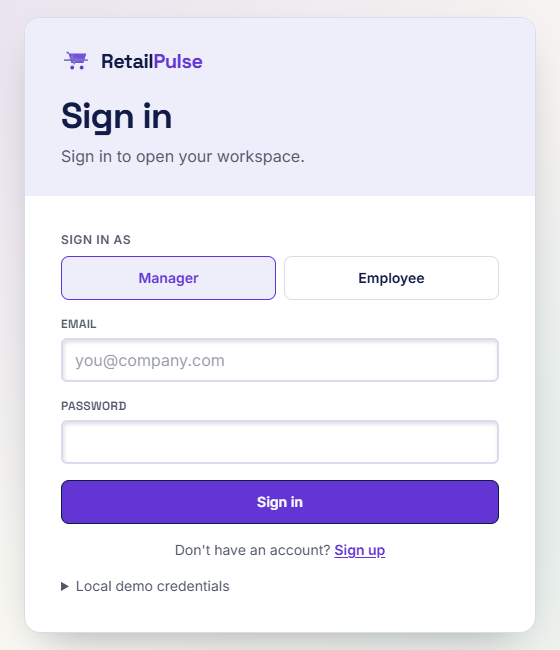
\includegraphics[width=0.42\textwidth]{ThesisFigs/ui_login.png}
\caption[Sign-in page]{Sign-in page. The user chooses the Manager or Employee workspace; a choice that does not match the stored role is refused (FR-02).}
\label{fig:ui-login}
\end{figure}

\begin{figure}[htbp]
\centering
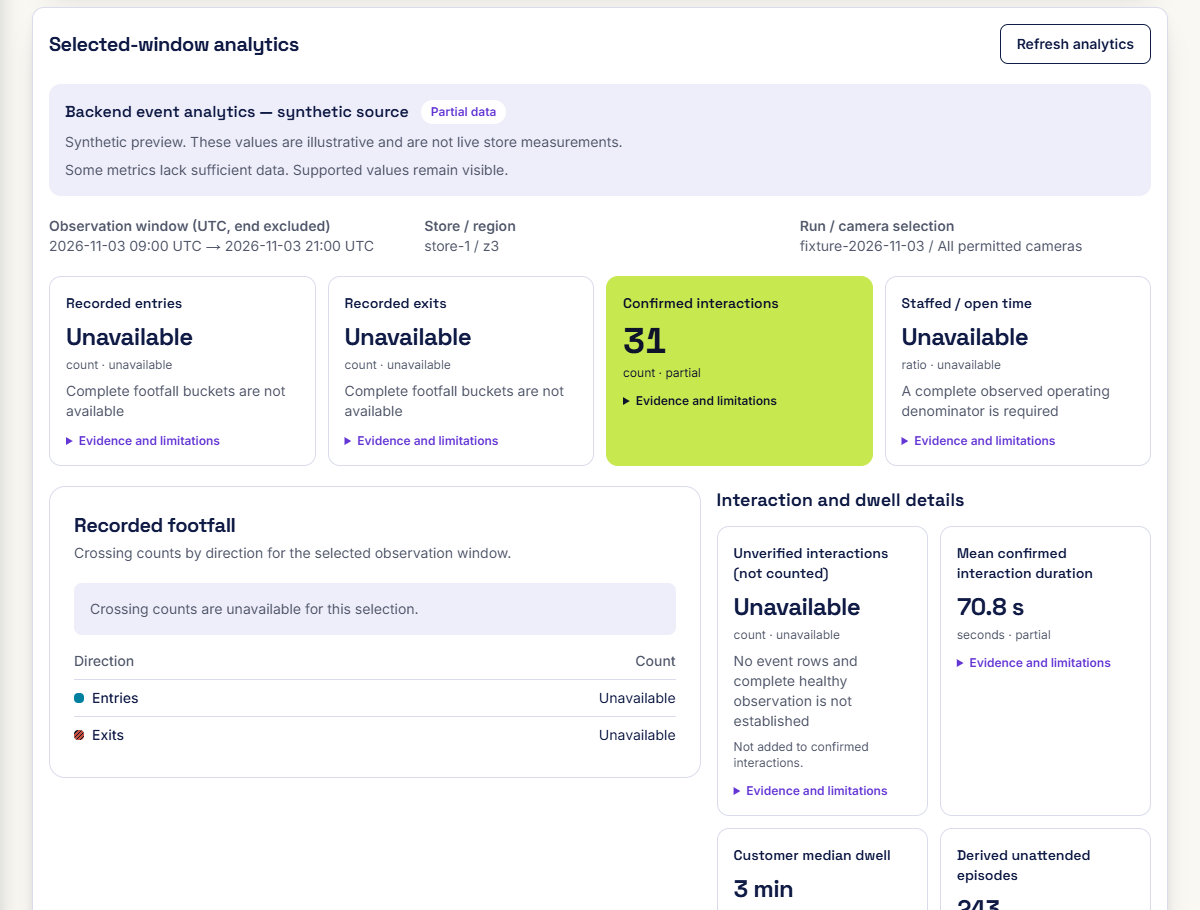
\includegraphics[width=\textwidth]{ThesisFigs/ui_dashboard.png}
\caption[Manager dashboard]{Manager dashboard for aisle z3 over the fixture day. The banner marks the source as synthetic and the data as partial; metrics without enough evidence (footfall, staffed share) are shown as unavailable with the reason rather than as zero (FR-17, NFR-06).}
\label{fig:ui-dashboard}
\end{figure}

\begin{figure}[htbp]
\centering
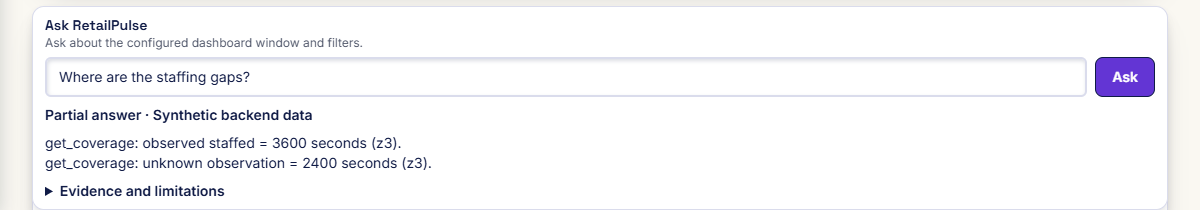
\includegraphics[width=\textwidth]{ThesisFigs/ui_ask.png}
\caption[Ask panel answering a staffing question]{Ask panel answering ``Where are the staffing gaps?''. Each line names the tool and metric it came from; the answer is marked partial because 2\,400 of the zone's seconds were unobserved (FR-18, FR-19).}
\label{fig:ui-ask}
\end{figure}

\begin{figure}[htbp]
\centering
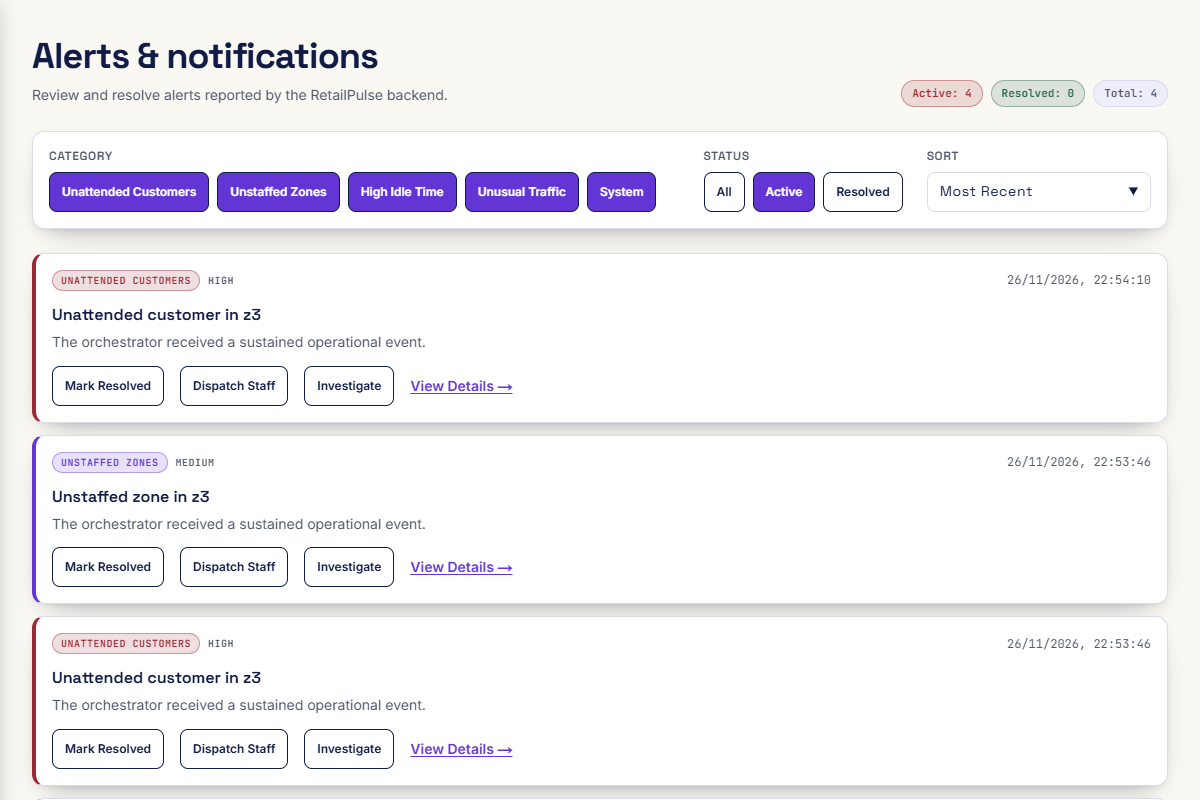
\includegraphics[width=\textwidth]{ThesisFigs/ui_alerts.png}
\caption[Alerts page]{Alerts page with the unattended-customer and unstaffed-zone events raised for aisle z3, filters by category and status, and actions to resolve, dispatch or investigate (FR-30).}
\label{fig:ui-alerts}
\end{figure}

\begin{figure}[htbp]
\centering
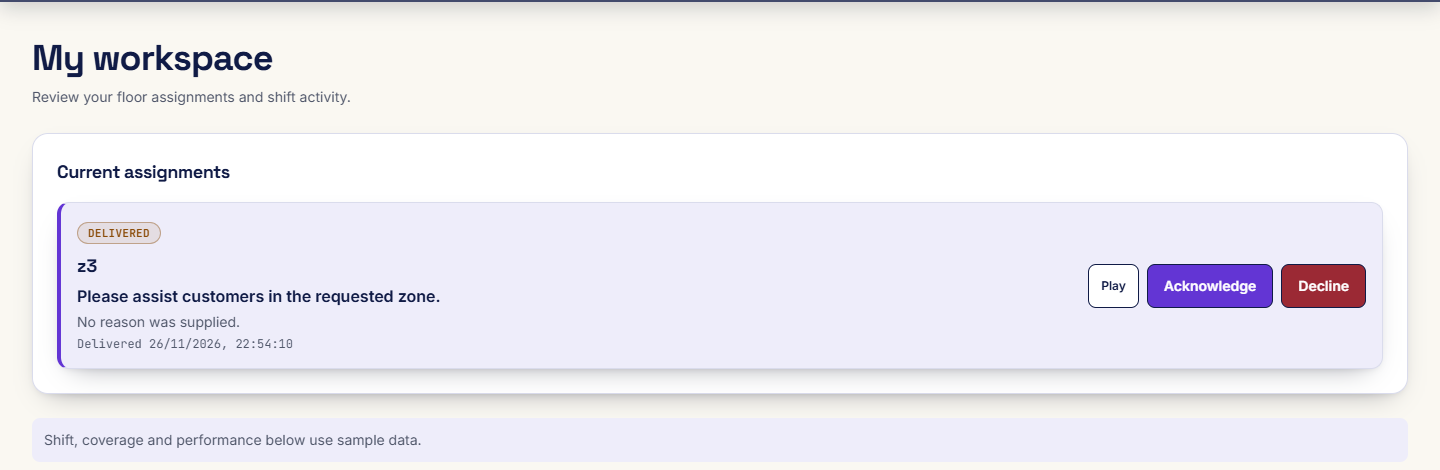
\includegraphics[width=\textwidth]{ThesisFigs/ui_employee_home.png}
\caption[Employee workspace with a dispatched task]{Employee workspace showing the task dispatched for aisle z3 in the \emph{delivered} state, with Play (spoken instruction), Acknowledge and Decline (FR-27 to FR-29). The shift cards below it use sample data and are labelled as such on the page.}
\label{fig:ui-employee}
\end{figure}

\begin{figure}[htbp]
\centering
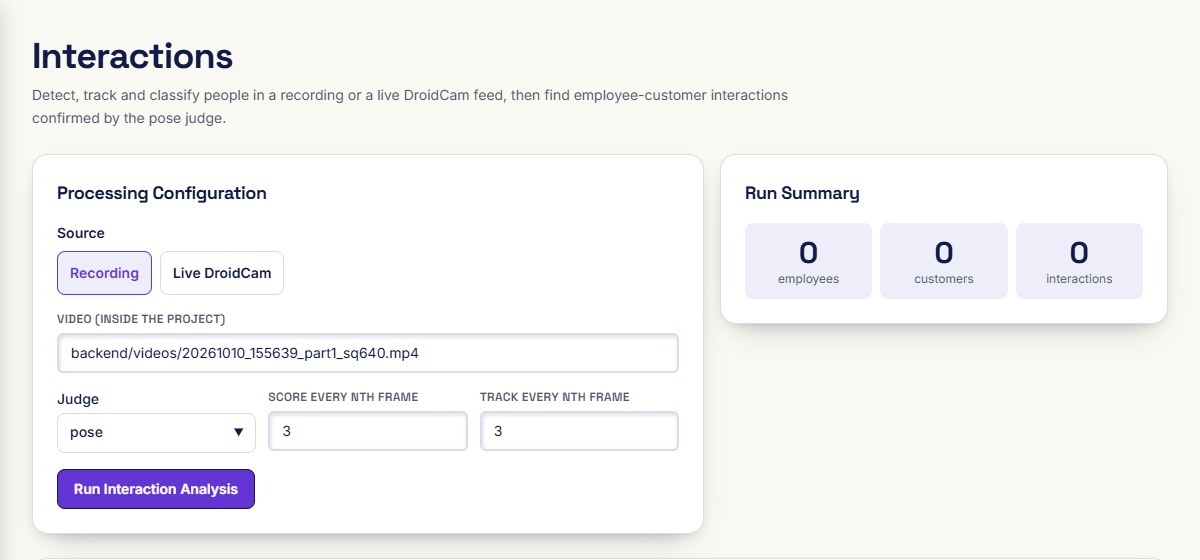
\includegraphics[width=\textwidth]{ThesisFigs/ui_interactions.png}
\caption[Interaction analysis page]{Interaction analysis page, where the manager starts a run on a recording or a live camera with the pose judge and sampling rates (UC-02).}
\label{fig:ui-interactions}
\end{figure}

\begin{figure}[htbp]
\centering
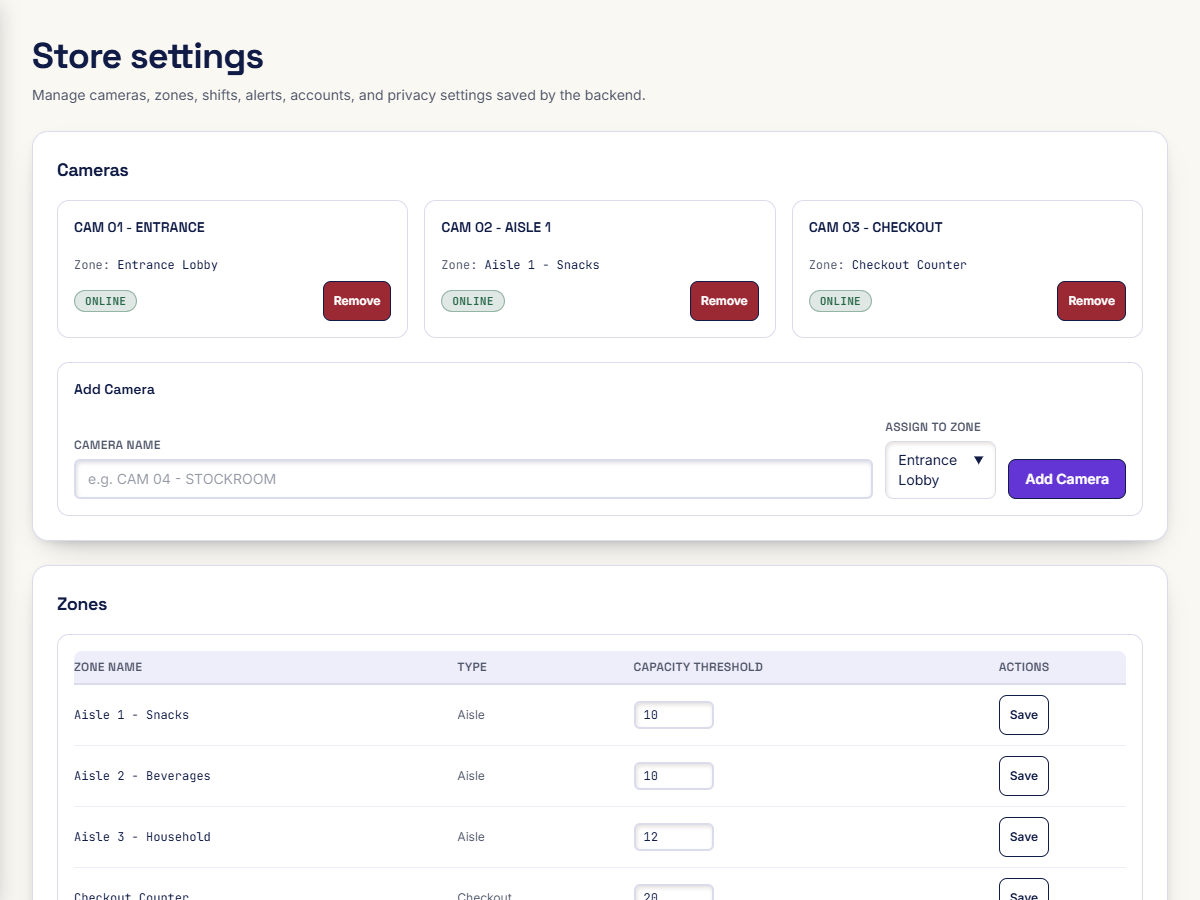
\includegraphics[width=\textwidth]{ThesisFigs/ui_settings.png}
\caption[Store settings]{Store settings for cameras and zones, saved by the backend (FR-31).}
\label{fig:ui-settings}
\end{figure}

\chapter{Evaluation of the Vision Pipeline}
\label{ch:cveval}

This chapter measures how well the pipeline detects people, classifies roles, finds interactions and how fast it runs. Every number names the report file it comes from; all files are in \path{backend/interaction/benchmarks/}. Numbers from clips the rules were tuned on are kept separate from numbers on held-out clips, and the headline result carries a confidence interval.

\section{Evaluation Method}
\subsection{Data}
Twenty-five labelled clips from one store and two cameras were split into two sets:
\begin{itemize}
\item \textbf{Tuning set} (11 clips, \path{benchmark.json}): 13 interactions and 4 pass-bys. The interaction rules were tuned on these clips, so their scores are optimistic.
\item \textbf{Held-out set B} (14 clips, \path{benchmark_set_b.json}): 17 interactions and 9 pass-bys. Set B uses only recordings from the detector's test and validation split, so no set-B frame was used to train the detector. It was looked at once during tuning, to set the rule that merges interaction spans separated by short gaps.
\end{itemize}
Labels were drawn and reviewed in CVAT. Every person in the 25 clips was reviewed for role (\path{persons.json}); a pipeline track takes the role of the reviewed person whose box it overlaps (IoU $\geq 0.3$ in at least half of its frames), which matched 109 of 113 tracks. The tuning-set labels have a single annotator.

\subsection{Metrics}
A predicted interaction matches a labelled one when their time spans overlap with temporal IoU $\geq 0.5$, one to one. Because this strict matching counts one long prediction that covers several short labels as both a miss and a false alarm, a per-second overlap score is reported as well. 95\,\% confidence intervals use a bootstrap over clips with 10\,000 resamples and a fixed seed~\cite{efron1979bootstrap}. Speed is the real-time factor: seconds of video processed per second of computation on a CPU.

\section{Results}
Table~\ref{tab:cv-results} gives the results with the fitted role weights adopted on 14 November 2026 (Section~\ref{sec:role-weights}). The headline is F1~0.450 on held-out set B, with a 95\,\% interval of 0.26--0.63; it meets the NFR-02 target of 0.40, although the lower end of the interval does not.

\begin{longtable}{P{0.19\textwidth}P{0.14\textwidth}P{0.26\textwidth}P{0.22\textwidth}P{0.11\textwidth}}
\caption{Vision pipeline results (fitted role weights unless stated)}\label{tab:cv-results}\\
\toprule
Stage & Metric & Set B (held out) & Tuning set & Source\\
\midrule
\endfirsthead
\toprule
Stage & Metric & Set B (held out) & Tuning set & Source\\
\midrule
\endhead
\bottomrule
\endfoot
Detector (best\_320, OpenVINO, 455 test images) & mAP50 / mAP50--95 / P / R & 0.969 / 0.896 / 0.963 / 0.953 & same detector & detector report\\
Interactions, proximity only & P / R / F1 & 0.346 / 0.529 / 0.419 (TP 9, FP 17, FN 8) & 0.619 / 1.000 / 0.765 & fitted reports\\
Interactions, with pose check & P / R / F1 & \textbf{0.391 / 0.529 / 0.450} (TP 9, FP 14, FN 8) & 0.765 / 1.000 / 0.867 (TP 13, FP 4, FN 0) & fitted reports\\
F1 95\,\% interval & with pose check & [0.261, 0.634] & [0.788, 0.960] & bootstrap\\
Per-second overlap & P / R / F1 & 0.521 / 0.943 / 0.671 & 0.711 / 0.904 / 0.796 & saved spans\\
Timing error & start / end (s) & 1.16 / 2.93 & 1.15 / 1.96 & reports\\
Roles & accuracy per track & 1.000 (56 tracks) & 0.957 (47 tracks) & fitted reports\\
Tracking & ID switches per minute & 1.68 & 2.04 & fitted reports\\
Speed & real-time factor (CPU) & \textbf{0.60$\times$} on an idle machine & & idle speed run\\
\end{longtable}

The fitted reports are \path{report_set_b_fitted_20261117.json} and \path{report_11_fitted_20261117.json}; the intervals are in \path{confidence_set_b_fitted_20261117.txt} and \path{confidence_11_fitted_20261117.txt}; the detector report is \path{report_set_b_merged.json} and the idle speed run is \path{report_set_b_speed_idle.json}. The per-second and timing rows come from the earlier run with hand-set role weights (\path{report_set_b_merged.json}, \path{report_11_merged.json}) and were not recomputed for the fitted run.

\paragraph{The pose check.} In the same run, the pose check removes 3 of the 17 proximity-only false positives on set B without losing a true positive, so precision rises from 0.346 to 0.391 and F1 from 0.419 to 0.450. On the tuning set it halves the false positives (8 to 4). Recall cannot change, because the check can only veto candidates.

\paragraph{Tuning set against held-out set.} F1 falls from 0.867 on the tuning clips to 0.450 on set B, and the two intervals do not overlap. This is the cost of tuning rules on a small set and the reason set B is the headline. The per-second recall of 0.943 on set B shows that most labelled interaction time is covered by some prediction: the pipeline usually finds the pair but draws the start and end differently from the labeller (Section~\ref{sec:cv-errors}).

\paragraph{Speed.} On an idle machine the pipeline processes set B at 0.60 times real time on a CPU (median 95\,ms per frame; the pose check costs 240--320\,ms per candidate pair), and up to about 1.5 times real time on individual clips. This meets NFR-01 (0.5 times real time). Runs that shared the CPU with other work measured 0.09--0.48 times and are not valid speed results. No GPU was available.

\section{Role Weights}
\label{sec:role-weights}
Each track's role is a weighted sum of employee evidence compared with a threshold. The original hand-set weights were reference similarity 0.55, bib colour 0.30, staff zone 0.10 and standing still 0.05, with a threshold of 0.45; on an uncalibrated camera the reference weight passes to the role detector's vote. A logistic regression with leave-one-clip-out validation was compared with them (Table~\ref{tab:roles}).

\begin{table}[H]
\centering
\caption{Hand-set against fitted role weights, leave-one-clip-out}\label{tab:roles}
\begin{tabular}{P{0.2\textwidth}P{0.15\textwidth}P{0.22\textwidth}P{0.13\textwidth}P{0.22\textwidth}}
\toprule
Set & Hand-set accuracy & Hand-set employee recall & Fitted accuracy & Source\\
\midrule
Tuning set (50 tracks) & 0.960 & 0.889 & 1.000 & \path{refit_benchmark/}\\
Set B (59 tracks) & 0.915 & 0.815 (misses 5 of 27) & 1.000 & \path{refit_benchmark_set_b/}\\
\bottomrule
\end{tabular}
\end{table}

The fit puts almost all weight on the role detector's vote (0.61) and bib colour (0.36), a little on standing still, and none on reference similarity or staff zones, with a threshold near 0.09 (\path{store_roles_fitted.json}). The zero weights mean those cues never occurred in the clips, because no camera is calibrated and no staff zone is drawn; they do not show the cues are useless. Figure~\ref{fig:role-sweep} shows that the fitted weights keep full employee recall over a wide range of thresholds, while the hand-set recall falls once the threshold passes about 0.2.

\begin{figure}[htbp]
\centering
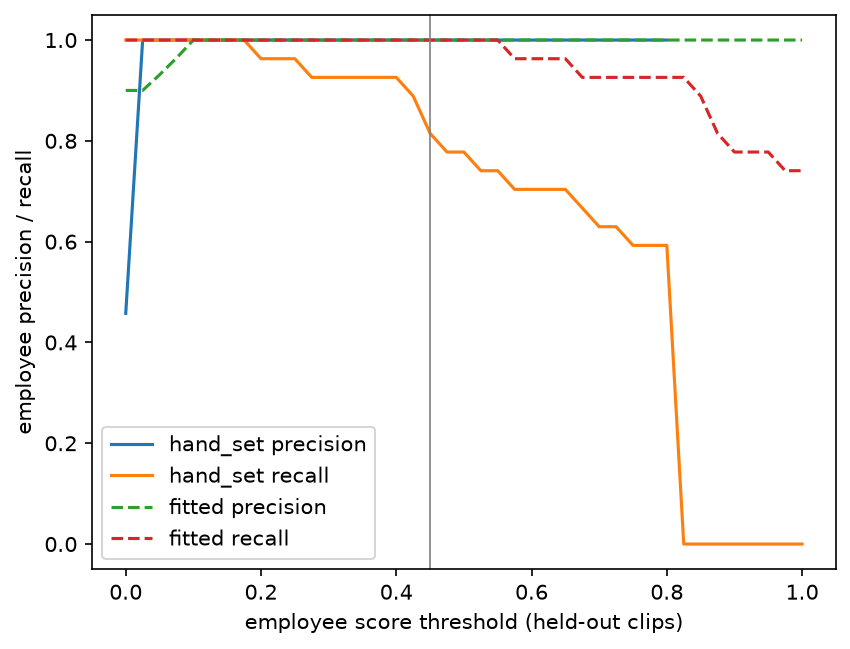
\includegraphics[width=0.62\textwidth]{ThesisFigs/role_threshold_sweep_set_b.png}
\caption[Role threshold sweep on held-out set B]{Employee precision and recall against the decision threshold on held-out set B: hand-set weights (solid) and fitted weights (dashed). The grey line is the hand-set threshold of 0.45.}
\label{fig:role-sweep}
\end{figure}

\textbf{Decision.} The fitted weights were adopted on 14 November 2026 and both benchmark specifications now load them for every clip. With them, role classification is correct for all 56 matched set-B tracks, meeting NFR-03. With two cameras and few clips this is not a general accuracy claim, and a store whose cameras are calibrated or have staff zones must refit the weights.

\section{Error Analysis}
\label{sec:cv-errors}
All false positives and misses on set B were inspected frame by frame (13 false positives and 8 misses in the hand-set run; the fitted run adds one false positive). They fall into three groups.
\begin{enumerate}
\item \textbf{Spans too long (4 false positives, 6 misses).} One prediction covers several shorter labelled interactions; on clip 155639 a prediction from 9.7 to 38.3\,s covers labels at 11.2--15.8, 19.5--28.4 and 34.3--36.7\,s. The 4\,s gap bridge joins what the labeller kept apart. The pair is found; the open question is whether a pause of 4--6\,s ends an interaction.
\item \textbf{Duplicates after a customer identity switch (4 false positives).} When the tracker gives a customer a new identifier mid-interaction, the merge cannot join the halves. The fix belongs in tracking, not in the merge rule.
\item \textbf{No label nearby (5 false positives).} Two look like missed labels (on IMG\_8838 part~2 the pair face each other for about 28\,s; on IMG\_8830 a customer gestures at a seated employee). One is two employees talking, and two are people side by side without engaging.
\end{enumerate}
If a blind re-check confirms the two suspected missed labels, set-B F1 would rise to about 0.49. Until that re-check is done, the reported figure is unchanged.

\section{Limitations}
\label{sec:cv-limits}
\begin{itemize}
\item \textbf{Small sample:} 30 labelled interactions in 25 clips from one store and two cameras; the interval on set-B F1 is wide (0.26--0.63).
\item \textbf{One look at set B} during tuning, to set the span merge.
\item \textbf{Identity switches} (1.7 per minute on set B) cause duplicate spans; no tracking fix has been made.
\item \textbf{Zone-level signals} (dwell per zone, entrance footfall, queues) are validated only on the synthetic fixture, because no camera has a registered map yet.
\item \textbf{Camera handoff} across cameras is implemented and unit-tested but not evaluated, because no crossings are labelled.
\item \textbf{Single annotator} for the tuning set; pass-bys are judgement calls.
\item \textbf{Detector scores} were not rerun with the fitted weights, because the detector test images are not on the evaluation machine; the detector is unchanged.
\end{itemize}

\chapter{Testing and Validation}
\label{ch:testing}

\section{Test Strategy}
Testing works at five levels, each with a different kind of evidence:
\begin{enumerate}
\item \textbf{Unit tests} check single modules with known inputs: role decisions, the pose judge, interaction nomination, signal policy rules, occupancy classification, grounding and narration.
\item \textbf{Database integration tests} run the readers, ingestion, dispatch and security code against a real PostgreSQL instance. Each test creates its own temporary schema and drops it afterwards, so tests never share or damage data.
\item \textbf{Evaluation benchmarks} score the vision pipeline against labelled clips (Chapter~\ref{ch:cveval}), the question path against a golden set, and dispatch against a set of staffing scenarios.
\item \textbf{End-to-end rehearsal} runs the ten acceptance scenarios through the integrated code on a synthetic store day.
\item \textbf{Review and QA} covers what automated tests cannot: a security code review, a dashboard QA pass and manual browser checks.
\end{enumerate}
Synthetic and real evidence are never mixed: every result from the fixture day is labelled synthetic and is not reported as a store result.

\section{Automated Test Results}
\begin{table}[H]
\centering
\caption{Automated test suites}\label{tab:suites}
\begin{tabular}{P{0.25\textwidth}P{0.38\textwidth}P{0.28\textwidth}}
\toprule
Suite & Scope & Last recorded result\\
\midrule
Fast backend (CI job 1) & Agents, tools, graph, business agents, events, dispatch, operations, security, PostgreSQL migration & 276 passed (17 Nov 2026, PostgreSQL 17)\\
Frontend (CI job 2) & Provider, controller, dashboard rendering, session and identity; lint, type check and production build & 40 passed; type check and lint pass (17 Nov 2026)\\
Vision (CI job 3) & Detector, tracker, role classifier, engagement, judge, benchmark metrics, refit, confidence & Passes in CI (run \#24)\\
Golden questions & 51 questions through the real router and graph on the fixture day & Routing 1.0, answers 1.0, refusals 1.0, grounded runs 1.0\\
Dispatch scenarios & 20 staffing scenarios through the real dispatch code & All 20 run; agreement with a human rater pending\\
\bottomrule
\end{tabular}
\end{table}

All three CI jobs passed on the integration branch. A separate run by the team on 14 November 2026 against the hosted Neon database also passed (223 passed, 2 skipped for a missing optional library), which confirmed the tests work against the production database service and not only the CI container. Appendix~\ref{app:tests} lists the test files by area.

\textbf{Golden questions.} On the first run of the 51-question set, routing accuracy was 0.941, answer accuracy 0.922 and refusal accuracy 0.917; every run that produced an answer was fully grounded. The failures were fixed, for example ``Who is the worst performing employee?'' is now refused and ``Where are the staffing gaps?'' is now routed. The perfect second-run score is measured on the same questions the fixes were written for, so it is not an independent result.

\textbf{Dispatch scenarios.} The 20 scenarios cover one free employee, a busy target-zone employee with a free floater, protection of zone minimum staffing, unrostered staff, nobody available, ranking between floaters and spare staff, and tie-breaks. The system's choices are recorded. They will be compared with a human rater's blind choices, collected on a rating sheet that hides the expected answers, before the agreement figure is reported.

\section{Acceptance Scenarios}
Ten end-to-end acceptance scenarios were defined (Table~\ref{tab:acceptance}). A scenario passes only on real footage through the integrated system; none has yet been run on real footage. To prove the wiring before that, all ten were rehearsed through the real code paths on the synthetic fixture day against PostgreSQL (\path{python -m backend.acceptance_rehearsal}). The rehearsal passed eight; the other two cannot run without inputs that do not exist yet.

\begin{longtable}{P{0.05\textwidth}P{0.2\textwidth}P{0.42\textwidth}P{0.23\textwidth}}
\caption{Acceptance scenarios and synthetic rehearsal (17 November 2026)}\label{tab:acceptance}\\
\toprule
ID & Scenario & Pass condition & Rehearsal\\
\midrule
\endfirsthead
\toprule
ID & Scenario & Pass condition & Rehearsal\\
\midrule
\endhead
\bottomrule
\endfoot
A1 & Clip to events & Rows in every event table with run, store and camera identifiers; \texttt{validate()} returns no problems; health covers the clip & Pass (720 of 720 minutes per camera)\\
A2 & Events to map & Each cell carries a map version; unmapped areas are marked & Not runnable: no floor plan or calibration points supplied\\
A3 & Live categories & Customer becomes \emph{no one} only after the hold; staff with a customer shows both; a covered lens gives insufficient coverage, never \emph{no one} & Pass\\
A4 & Manager question & Real agents (not stubs); every number equals a tool metric; caveats shown & Pass\\
A5 & Unattended to employee & Event raised, real handler called, eligible employee gets a task, manager sees it & Pass\\
A6 & No eligible employee & Outcome \emph{no eligible employee}; no task; manager alerted & Pass\\
A7 & Duplicate event & Same key; outcome \emph{duplicate}; still one task & Pass\\
A8 & Blind camera & Event suppressed for unknown observation; no task & Pass\\
A9 & Digest & Figures verified; provenance labelled; caveat names the blind interval & Pass\\
A10 & Clip review precision & Two reviewers; precision and Cohen's kappa recorded & Not runnable: needs two human reviewers and recordings\\
\end{longtable}

The rehearsal found and fixed three defects before this report: the router refused A4's own question ``Where are the staffing gaps?'', the narrative check treated the digits in zone identifiers such as \texttt{z3} as figures, and the digest's coverage caveat did not say when the camera was blind. Each fix has a regression test.

\section{Non-Functional Requirement Verification}
\begin{longtable}{P{0.1\textwidth}P{0.34\textwidth}P{0.29\textwidth}P{0.17\textwidth}}
\caption{Verification of non-functional requirements}\label{tab:nfr-verify}\\
\toprule
ID & Target & Evidence & Status\\
\midrule
\endfirsthead
\toprule
ID & Target & Evidence & Status\\
\midrule
\endhead
\bottomrule
\endfoot
NFR-01 & $\geq 0.5\times$ real time on CPU & 0.60$\times$ on an idle machine & Met\\
NFR-02 & Interaction F1 $\geq 0.40$ held out & 0.450, interval 0.26--0.63 & Met (point estimate)\\
NFR-03 & Role accuracy $\geq 95\,\%$ held out & 100\,\% of 56 tracks & Met\\
NFR-04 & Replay creates no task & A7; dispatch unit tests & Met (synthetic)\\
NFR-05 & Every event row valid & \texttt{validate()} in A1 and on each run & Met\\
NFR-06 & Missing coverage never shown as empty & A3, A8; occupancy tests & Met (synthetic)\\
NFR-07 & PBKDF2 $\geq$ 600\,000 iterations; 8-character passwords & Security tests & Met\\
NFR-08 & Secret required; no default secrets & Security tests; startup refusal & Met\\
NFR-09 & 10 questions per minute & Ask API test & Met (per process)\\
NFR-10 & No biometric or account-linked identity stored & Schema and code review & Met by review\\
NFR-11 & Two navigation actions; no horizontal scroll at 390\,px & Dashboard QA; mobile checks & Partly verified\\
NFR-12 & Three CI jobs on every push & Workflow runs & Met; branch protection not yet enabled\\
NFR-13 & Thresholds configurable without code & Policy and settings tests & Met\\
\end{longtable}

\section{Known Defects and Open Issues}
\begin{itemize}
\item The backend accepts any listed task state from any state; the order of task transitions is not enforced.
\item Ingestion of a run started from the web page is a separate command, not automatic.
\item The Ask rate limit is per process; a shared database budget exists but its schema has not been applied to a deployment.
\item Branch protection on the main branch is not enabled, so passing CI is not yet required before a merge.
\item No scenario has been accepted on real store footage, and the backend has not been deployed.
\end{itemize}

\chapter{Project Management}
\label{ch:mgmt}

\section{Development Approach}
The project follows an iterative process. Each iteration ends with a working, tested increment and a review of what to keep, change or drop; the floor-distance prototype, for example, was dropped after iteration~1 when moving-camera footage showed it could not work. Work is split into owned work items (for example B1 labels, C3 dispatch, M-UI-P3 dashboard connection), each developed on a feature branch, reviewed and merged into a shared integration branch. Status, contracts and open items are kept in tracked planning documents in the repository so every member works from the same information.

\section{Timeline and Milestones}
\begin{longtable}{P{0.2\textwidth}P{0.72\textwidth}}
\caption{Milestones}\label{tab:milestones}\\
\toprule
Date & Milestone\\
\midrule
\endfirsthead
\toprule
Date & Milestone\\
\midrule
\endhead
\bottomrule
\endfoot
26 Aug 2026 & First commit to the repository\\
11 Sep 2026 & Proposal defence (feedback in Appendix~\ref{app:feedback})\\
12 Oct 2026 & Supervisor accepts the team's 70-video dataset\\
21 Oct 2026 & Mid evaluation: vision prototype and web application (iteration~1)\\
24 Oct 2026 & Model consolidation: COCO detector tracks everyone, role detector only labels\\
3 Nov 2026 & Iteration~2 begins with the team's 16-week plan\\
5--8 Nov 2026 & 25 clips labelled; benchmarks on tuning and held-out sets\\
10 Nov 2026 & Agent foundation: typed tools, scoped registry, orchestration graph\\
11 Nov 2026 & Move to PostgreSQL; dashboard connected to the backend\\
12 Nov 2026 & Business agents, signal policy, occupancy categories, digest, clip review, CI workflow\\
13 Nov 2026 & Security fixes; direct dispatch connected end to end\\
14 Nov 2026 & Role-weight decision; acceptance rehearsal on the hosted database\\
15--18 Nov 2026 & Map registration, directional footfall, frontend security, production audit\\
17 Nov 2026 & Benchmarks rerun with fitted weights; 276 backend tests\\
25--26 Nov 2026 & Aisle relay demonstration; dispatch skips employees in an interaction\\
\end{longtable}

\section{Team Responsibilities}
\begin{table}[H]
\centering
\caption{Ownership of components}\label{tab:ownership}
\begin{tabular}{P{0.2\textwidth}P{0.72\textwidth}}
\toprule
Member & Responsibilities\\
\midrule
Moiz Ansari (23I-0523) & Manager frontend and dashboard binding; agent foundation (typed tools, scoped registry, orchestration graph, operational adapter); Ask route; footfall counter; PostgreSQL migration\\
Saqib Atif (23I-0769) & Vision pipeline, labelling and benchmarks; event store and ingestion; dispatch and voice; map registration; security fixes; aisle relay demonstration\\
Ruhab Ahmad (23I-0559) & Employee frontend; Customer Behavior and Employee Activity agents; signal policy; occupancy categories; digest; clip review; golden questions; acceptance tests; security review; CI workflow; role-weight decision; documentation and this report\\
\bottomrule
\end{tabular}
\end{table}

\section{Version Control Evidence}
The repository \path{muhammad-moiz-ansari/retail-store-analysis} has 339 commits on the branch described here, from 26 August to 26 November 2026. Git records them under five author identities: Moiz Ansari (136), \texttt{msaqibatifj} (128) and Muhammad Saqib Atif (2) for Saqib, Ruhab Ahmad (62), and \texttt{GulsherKhan-04} (11). The last identity holds Saqib's labelling and benchmark commits of 5--8 November, which were recorded under the wrong identity and re-authored to him on the shared integration branch. Commit counts measure activity, not the size or value of each contribution.

\section{Risk Management}
\begin{longtable}{P{0.22\textwidth}P{0.34\textwidth}P{0.36\textwidth}}
\caption{Risks and responses}\label{tab:risks}\\
\toprule
Risk & Effect & Response\\
\midrule
\endfirsthead
\toprule
Risk & Effect & Response\\
\midrule
\endhead
\bottomrule
\endfoot
No store would share footage & No data to train or evaluate & Team recorded its own 70-video dataset, accepted by the supervisor\\
No GPU & Slow processing & Small models, OpenVINO, frame sampling and role labelling only for new tracks; 0.60$\times$ real time achieved\\
Moving cameras & Floor mapping failed & Floor prototype descoped; body-height distance used\\
Small labelled set & Unreliable accuracy figures & Held-out set, bootstrap intervals, error analysis, blind re-check planned\\
Language model invents figures & Wrong answers to managers & Claims must cite tool metrics; grounding and narrative checks; model used only for routing\\
Duplicate or wrong dispatch & Staff sent twice or a zone left empty & Unique event key; eligibility protects minimum staffing; scenario tests\\
Exposed secrets & Forged sessions & Startup refuses default secrets; secrets server-side; keys exposed earlier are being rotated\\
Store map not supplied & Map-cell occupancy cannot be shown & Map registration tested on synthetic geometry; real map requested for FYP-2\\
\end{longtable}

\section{Tools and Generative-AI Use}
Development used Git and GitHub, GitHub Actions, CVAT for labelling, Node.js, a Python virtual environment and PostgreSQL. Generative-AI assistants were also used, as disclosed in Table~\ref{tab:ai-use}. Every AI-assisted change was checked by tests and by the member who owns the affected component, and each member must be able to explain the code and text in their area.

\begin{table}[H]
\centering
\caption{Generative-AI use and how it was checked}\label{tab:ai-use}
\begin{tabular}{P{0.15\textwidth}P{0.4\textwidth}P{0.37\textwidth}}
\toprule
Tool & Used for & Check\\
\midrule
Claude Code & Implementation support for agents, tests, acceptance rehearsal, report drafting and figure redrawing & Automated tests; benchmark reruns; every report number traced to its source file; figures checked against the code\\
Codex & Implementation support for the descoped floor prototype and documentation & Automated tests and output inspection\\
Claude & General development questions & Review by the owning member\\
\bottomrule
\end{tabular}
\end{table}

\chapter{Conclusion and Future Work}
\label{ch:conclusion}

\section{Conclusion}
RetailPulse set out to turn the footage a store already records into service and staffing information on an ordinary CPU, without identifying anyone. At the end of FYP-1 the core loop works end to end on recorded and synthetic data: the vision pipeline finds people, labels customers and employees, and confirms interactions with a pose check; each run becomes validated events in PostgreSQL; two business agents answer manager questions with figures that are checked against their source; and an unattended customer becomes a task for an eligible employee, without a manager approval step and never twice for the same event.

Measured against the objectives of Chapter~\ref{ch:intro}:
\begin{itemize}
\item \textbf{O1, roles:} all 56 matched held-out tracks classified correctly with the fitted weights.
\item \textbf{O2, interactions:} F1 0.450 on held-out clips (interval 0.26--0.63); the pose check raises precision from 0.346 to 0.391 at equal recall.
\item \textbf{O3, event store:} every run's rows pass the contract check; a synthetic day covers all event tables.
\item \textbf{O4, questions:} 51 golden questions are routed, answered and refused correctly, with every answer fully grounded (after fixes made on the same set).
\item \textbf{O5, dispatch:} dispatch, no eligible employee, duplicates and blind cameras behave correctly in tests and in the synthetic rehearsal.
\item \textbf{O6, CPU only:} 0.60 times real time on an idle CPU.
\item \textbf{O7, access:} the security review's findings are fixed and tested.
\end{itemize}

The mid evaluation found the report's figures and requirements incorrect. This report rebuilds both: the requirements specification is now numbered, atomic and testable with measurable non-functional targets, and every design figure has been redrawn from the current code.

The main limitation is evidence, not function: no acceptance scenario has yet passed on real store footage, the backend has not been deployed, and the labelled set is small enough that the accuracy interval is wide.

\section{FYP-2 Plan}
\begin{longtable}{P{0.27\textwidth}P{0.45\textwidth}P{0.2\textwidth}}
\caption{FYP-2 work plan}\label{tab:fyp2}\\
\toprule
Work & Done when & Owner\\
\midrule
\endfirsthead
\toprule
Work & Done when & Owner\\
\midrule
\endhead
\bottomrule
\endfoot
Real-footage acceptance & A1--A10 pass on recorded store footage through the integrated system & Ruhab (lead), all\\
Store map and calibration & Floor plan and camera points supplied and registered; A2 runs; map view shows real cells & Saqib, Moiz\\
Backend deployment & Backend reachable from the deployed web tier with production secrets; S1 checked in the deployment & Saqib\\
Automatic ingestion & A run started from the web page is stored without a manual command & Saqib\\
Second annotator and blind re-check & Tuning labels second-reviewed; IMG\_8838 part~2 and IMG\_8830 re-checked & Labeller, Ruhab\\
Dispatch agreement & Human rater's blind choices compared with the system on all 20 scenarios & Ruhab\\
Clip review on real events & Two reviewers; precision and Cohen's kappa reported (A10) & Ruhab, Saqib\\
Task transitions & Backend rejects out-of-order task states & Saqib\\
Camera handoff & Labelled crossings collected and the handoff evaluator scored & Saqib\\
Branch protection & CI required before merging to the main branch & Moiz\\
Model and agent freeze & Weights and configuration frozen and recorded before the final demonstration & All\\
\end{longtable}

\section{Future Work Beyond FYP-2}
Cross-camera re-identification without biometric identity, metric floor distances with calibrated static cameras, GPU deployment for real-time processing, shelf-level product interaction, and operation across several stores remain outside the project scope. They are recorded so a later project can start from the same event store and agent contracts.


\appendix
\chapter{Evaluation Feedback and Responses}
\label{app:feedback}

\section{Mid Evaluation (21 October 2026)}
\begin{quote}
Reports need improvement. Figures were incorrect, and the SRS is incorrect.
\end{quote}

\subsection{Figures}
Every design figure was redrawn for this report from the current code. Table~\ref{tab:fig-fixes} lists what was wrong with each mid-report figure and how its replacement differs.

\begin{longtable}{P{0.18\textwidth}P{0.4\textwidth}P{0.34\textwidth}}
\caption{Mid-report figures and their replacements}\label{tab:fig-fixes}\\
\toprule
Figure & Problem in the mid report & Replacement\\
\midrule
\endfirsthead
\toprule
Figure & Problem in the mid report & Replacement\\
\midrule
\endhead
\bottomrule
\endfoot
Architecture & Drew the agents as one straight chain, each feeding the next, which the system never did; showed no data store, interfaces or security boundary & Layered architecture with the proxy, application, agent, vision and data layers, and every write path to the database (Figure~\ref{fig:architecture})\\
Domain model & Mixed software agents (``\guillemotleft agent\guillemotright'', ``\guillemotleft LLM'' with an unclosed stereotype) with problem concepts; association names cut off; overlapping multiplicities such as ``0..10..11..*''; dense line crossings & Problem concepts only, named associations with readable multiplicities (Figure~\ref{fig:domain})\\
Class diagram & Attributes shown only as types (``+String'') with no names; operations with no return types; planned agents and database tables mixed in one diagram & Two class diagrams of real classes with named, typed attributes and typed operations (Figures~\ref{fig:class-vision} and~\ref{fig:class-agents})\\
Deployment & Showed SQLite, which the system no longer uses; no event store, agents or hosted deployment; labels over boxes & Current deployment: Vercel, CPU application host, hosted PostgreSQL, optional services (Figure~\ref{fig:deployment})\\
Use cases & Four separate diagrams, no include or extend relations, an internal evaluation tool shown as a user goal & One diagram with twelve user-goal use cases and correct relations (Figure~\ref{fig:uc-diagram})\\
Dashboard screenshot & Old interface with demo data showing 38 entries, 42 exits and ``net inside $-4$'', an impossible negative occupancy & New screenshots of the current interface, taken from the running system with every figure coming from the backend and synthetic data labelled on screen (Section~\ref{sec:ui})\\
\end{longtable}

New figures were added for behaviour that the mid report did not model: the pipeline and orchestration flows, the database tables, two sequence diagrams and the task state machine.

\subsection{Software Requirements Specification}
The requirements chapter was rewritten (Chapter~\ref{ch:srs}). Appendix~\ref{app:req-changes} gives the detailed changes and maps the old requirement identifiers to the new ones.

\section{Proposal Defence (11 September 2026)}
The team recorded this feedback after the defence; no signed form is attached.
\begin{quote}
Students have no clue what they are doing. Technical knowledge is lacking. The students do not have an understanding of the project. Students need to learn more about the requirements of the project and next time be well prepared. Should work on their presentation skills; the presenters kept pacing back and forth. Their project was poorly explained, there was no clarity on the exact features, and the overall idea was unclear. Also, they did not defend the generalizability of their project; the behavioral requirements of employees vary from retail to retail store (for example, luxury brands like Gucci, Prada, etc. don't want their employees to be constantly approaching customers), so how is their project universal for all types of retail stores? Improve your skills. It is a healthy project if it is properly focused.
\end{quote}

\begin{table}[H]
\centering
\caption{Responses to the proposal-defence feedback}\label{tab:defence-response}
\begin{tabular}{P{0.3\textwidth}P{0.62\textwidth}}
\toprule
Point & Response\\
\midrule
Unclear features and requirements & Twelve use cases and 34 numbered, testable requirements (Chapter~\ref{ch:srs}); each requirement traced to design and tests\\
Technical understanding & Each member owns named components (Table~\ref{tab:ownership}) and their tests; results are reproducible from named files and commands\\
Generalisability across stores & Every waiting, staffing and coverage threshold is per-store configuration (constraint C3, NFR-13); a luxury store can raise the waiting threshold or pause dispatch without code changes\\
Focus & Out-of-scope features (re-identification, metric distance, shelf interaction) are stated explicitly; effort went to one complete loop from camera to task\\
\bottomrule
\end{tabular}
\end{table}

\chapter{Changes to the Requirements Specification}
\label{app:req-changes}

\section{Structural Changes}
\begin{enumerate}
\item \textbf{Numbering without gaps.} The mid report kept withdrawn identifiers, so its requirements ran FR-01, FR-02, FR-04, FR-07, FR-10 and so on. Requirements are now numbered FR-01 to FR-34 and grouped by module.
\item \textbf{One behaviour per requirement.} Several mid-report requirements combined many behaviours in one sentence (for example, footfall, exits and occupancy with coverage reporting). Each requirement now states one testable behaviour.
\item \textbf{Specification separated from progress.} The mid-report tables mixed requirements with implementation status (``Planned'', ``Partial'', ``honest evidence status''). The specification now states only what the system must do; progress and results are in Chapters~\ref{ch:impl} to~\ref{ch:testing}.
\item \textbf{Measurable non-functional requirements.} Mid-report NFRs had no targets, and one stated that no numeric target existed. Every NFR now has a measurable target and a verification method.
\item \textbf{Use cases are user goals.} ``Evaluate analytical outputs'' by an ``Operator / project team'' was an internal evaluation activity, not a goal of a store user; evaluation is now described as method in Chapter~\ref{ch:cveval}. The camera system was added as the actor that triggers dispatch, and include and extend relations are shown where they apply.
\item \textbf{Retired terms removed.} Hot and gray zones are no longer occupancy categories; the specification uses the four agreed categories and treats missing coverage as a quality mask.
\item \textbf{Added sections.} Product perspective with a context diagram, operating environment, constraints, external interfaces and a traceability table linking each requirement to design elements and tests.
\end{enumerate}

\section{Mapping of Mid-Report Requirements}
\begin{longtable}{P{0.11\textwidth}P{0.3\textwidth}P{0.18\textwidth}P{0.33\textwidth}}
\caption{Mid-report functional requirements and their replacements}\label{tab:fr-map}\\
\toprule
Old ID & Old capability & New IDs & Note\\
\midrule
\endfirsthead
\toprule
Old ID & Old capability & New IDs & Note\\
\midrule
\endhead
\bottomrule
\endfoot
FR-01 & Analyze a video & FR-05--FR-10 & Split into detection, tracking, roles, nomination, confirmation and outputs\\
FR-02 & Entrance footfall & FR-13 & Occupancy from footfall dropped: initial occupancy is unknown\\
FR-04 & Service interactions & FR-08, FR-09, FR-12 & Interaction nomination, pose confirmation, unattended episodes\\
FR-07 & Spatial customer activity & FR-15, FR-16 & Four occupancy categories replace hot and gray zones\\
FR-10 & Role-specific account & FR-01--FR-04 & Sign-in, role access, lockout, invitations\\
FR-11 & Monitor cameras & FR-14 & Camera health recorded per minute\\
FR-12 & Manager analytics & FR-17 & \\
FR-13 & Personal workspace & FR-28 & \\
FR-17 & Insight report with PDF export & FR-21 & Digest of verified figures; PDF export withdrawn\\
FR-18 & Operational alerts & FR-30 & \\
FR-19 & System status & FR-33 & \\
FR-20 & Personal settings & -- & Withdrawn: profile editing is not part of the delivered scope\\
FR-29 & Configure store & FR-31, FR-32 & Includes pausing dispatch\\
FR-34 & Evaluate outputs & -- & Moved to evaluation method (Chapter~\ref{ch:cveval})\\
FR-35 & Staff availability and coverage & FR-23, FR-24 & Unstaffed-zone events and suppression on unknown coverage\\
FR-36 & Aisle assignment & FR-22, FR-25--FR-29, FR-34 & Event, eligibility, ranking, delivery, status, duplicates\\
FR-37 & Analytics question & FR-18--FR-20 & Tools only, grounding, refusals\\
\end{longtable}

\chapter{Test Inventory}
\label{app:tests}
Test functions by area on commit \texttt{c8ff409}. Many tests are parametrised, so the number of executed cases is higher than the number of functions (276 cases in the fast backend job).

\begin{longtable}{P{0.36\textwidth}P{0.1\textwidth}P{0.46\textwidth}}
\caption{Test files and what they check}\label{tab:test-files}\\
\toprule
File & Tests & Checks\\
\midrule
\endfirsthead
\toprule
File & Tests & Checks\\
\midrule
\endhead
\bottomrule
\endfoot
\multicolumn{3}{l}{\textit{Business agents}}\\
\path{business/test_customer_behavior.py} & 10 & Intents, footfall paths, waiting customers, claims\\
\path{business/test_employee_activity.py} & 6 & Coverage and assistance answers\\
\path{business/test_signal_policy.py} & 6 & Emission, suppression and severity rules\\
\path{business/test_occupancy.py} & 9 & Four categories, masking, hysteresis, layers\\
\path{business/test_narration.py} & 6 & Digest sections, verified numbers, provenance\\
\path{business/test_clip_review.py}, \path{test_clip_render.py} & 8 & Blind review items, kappa, clip rendering\\
\path{business/test_golden.py} & 3 & Golden-question routing, answers, refusals\\
\multicolumn{3}{l}{\textit{Agent foundation}}\\
\path{agents/test_contracts.py} & 14 & Typed contracts reject malformed values\\
\path{agents/test_read_tools.py}, \path{test_contextual_tools.py}, \path{test_tool_integration.py} & 23 & Readers against PostgreSQL; scope enforcement\\
\path{agents/test_graph.py}, \path{test_graph_service.py} & 22 & Routing, grounding, repair, refusals, traces\\
\path{agents/test_operational.py}, \path{test_operational_integration.py} & 15 & Adapter validation; questions cannot reach dispatch\\
\path{agents/test_dashboard.py}, \path{test_ask_api.py}, \path{test_advisory_api.py} & 16 & Dashboard and Ask routes, membership, rate limit\\
\multicolumn{3}{l}{\textit{Events and operations}}\\
\path{events/test_events.py} & 11 & Ingestion, contract check, fixture day\\
\path{events/test_spatial.py}, \path{test_live_zones.py} & 16 & Map registration, cell dwell, camera attention state\\
\path{tests/test_dispatch.py}, \path{test_operations.py} & 14 & Eligibility, ranking, duplicates, scenarios, operations cycle\\
\path{tests/test_security.py} & 11 & Secrets, lockout, hashing, invitations, job limits, camera roles\\
\path{tests/test_aisle_relay.py} & 16 & Aisle relay watcher and store bridge\\
\path{tests/test_ack_time.py}, \path{test_task_voice.py}, \path{test_live_view.py} & 5 & Acknowledgement time, voice fallback, live view\\
\path{test_postgres_migration.py} & 3 & SQLite import into PostgreSQL\\
\multicolumn{3}{l}{\textit{Vision pipeline}}\\
\path{interaction/test_role_classifier.py}, \path{test_cust_emp_classifier.py} & 14 & Role labelling, rechecks, weighted decision\\
\path{interaction/test_engagement.py}, \path{test_judge.py} & 17 & Proximity nomination, pass-bys, pose verdicts\\
\path{interaction/test_tracker.py}, \path{test_identity.py} & 10 & Tracking and identity relinking\\
\path{interaction/test_benchmark.py}, \path{test_confidence.py}, \path{test_refit.py} & 14 & Metric calculations, bootstrap, refit\\
Other vision tests & 21 & CVAT import, role labels, renderer, live switch, task A, calibration\\
\path{test_handoff_core.py}, \path{test_handoff_eval.py} & 6 & Camera handoff logic and evaluator\\
\multicolumn{3}{l}{\textit{Frontend}}\\
Provider, controller, dashboard, session and identity tests & 40 & Validation, states, rendering, session signing, header stripping\\
\end{longtable}

\chapter{Meeting Record}
\label{app:meetings}
Supervisor: Mr.\ Shehreyar Rashid. Entries are recorded from the team's notes of each meeting.

\begin{longtable}{P{0.17\textwidth}P{0.38\textwidth}P{0.37\textwidth}}
\caption{Meetings and evaluations}\label{tab:meetings}\\
\toprule
Date & Discussion & Outcome\\
\midrule
\endfirsthead
\toprule
Date & Discussion & Outcome\\
\midrule
\endhead
\bottomrule
\endfoot
19 Aug 2026 & No dataset; retailers unwilling to share footage for privacy reasons & Supervisor advised the team to create its own dataset\\
8 Sep 2026 & Draft proposal-defence slides & Corrections requested before the defence\\
10 Sep 2026 & Client meeting & Details not recorded\\
11 Sep 2026 & Proposal defence & Feedback in Appendix~\ref{app:feedback}\\
5 Oct 2026 & Dataset progress & Deadline set for showing the dataset\\
12 Oct 2026 & Presentation of the 70-video dataset & Dataset accepted; no numeric accuracy target agreed\\
14 Oct 2026 & Progress update & Mid-evaluation date communicated\\
21 Oct 2026 & Mid evaluation & Figures and SRS found incorrect; addressed in this report (Appendix~\ref{app:feedback})\\
\end{longtable}


\bibliographystyle{IEEEtran}
\bibliography{references/references}
\end{document}
